\documentclass[10pt,a4paper]{article}
\usepackage{fontspec}
\usepackage[spanish,es-noshorthands,es-tabla]{babel}
\usepackage[margin=16mm]{geometry}
\usepackage{longtable,booktabs,array,graphicx,pdfpages,xcolor,tcolorbox}
\usepackage[hidelinks]{hyperref}
\usepackage{xurl}
\setlength{\parskip}{4pt}\setlength{\parindent}{0pt}\setlength{\tabcolsep}{3pt}
\renewcommand{\arraystretch}{1.1}
\newcolumntype{L}[1]{>{\raggedright\arraybackslash}p{#1}}
\newcommand{\ok}{\textcolor{green!45!black}{\textbf{OK}}}
\begin{document}
\begin{center}
{\LARGE\bfseries Sonómetro IEPE de 2 canales}\\[4pt]
{\Large Guía de conexiones para dibujar la Rev B en Altium}\\[6pt]
Universidad Nacional de Colombia, Manizales \quad · \quad 15 de noviembre de 2026
\end{center}
\begin{tcolorbox}[colback=green!4,colframe=green!40!black,title=Estado verificado]
La Rev B en KiCad (\texttt{hardware/pcb/}) tiene \textbf{125 componentes y 68 redes con nombre}.
Verificación automática: esquemático contra este diseño pin a pin \ok{} (0 diferencias), ERC \ok{} (0),
paridad PCB–esquemático \ok{} (0) y DRC sin errores. Lo único pendiente en la placa es el ruteo.
Fuentes: Altium \texttt{Sonometro\_2CH} del equipo, \texttt{docs/connection\_matrix.md} y los documentos
del fabricante citados en cada cambio.
\end{tcolorbox}

\section*{Cómo usar esta guía}
\begin{enumerate}
\item Abre el esquemático (sección~\ref{sec:esq}) junto a esta guía. Está dibujado por bloques: dentro de cada bloque
todo va con cables y entre bloques con etiquetas globales (puertos en Altium). Las alimentaciones van con
símbolos de alimentación (power ports): GND, 3V3, 5V, 5V\_A y 24V\_PROT.
\item Usa \textbf{exactamente las mismas referencias} (R1, U4, A1…) y \textbf{los mismos números de pin}.
Las piezas marcadas \textbf{NUEVO} no existen en la Rocket\_Library: hay que crear símbolo y footprint
(los footprints de KiCad sirven de referencia; los de JLC salen de su página con el código LCSC). Las marcadas
\emph{Gateway} están en el proyecto Altium del gateway (bucks): cópialas de ahí. En las piezas nuevas respeta
los números de pin de las tablas (p. ej. D1/D2: 1 = cátodo K, 2 = ánodo A; BNC: 1 = centro, 2–4 = carcasa).
\item Proyecto \textbf{plano}, como el del equipo: entre hojas une los bloques con \emph{Ports} o
\emph{Power Ports}; un \emph{Net Label} solo vale dentro de su propia hoja.
\item El zócalo de la NUCLEO (A1) es \textbf{un solo componente de 30 pines}: 1–15 = CN3-1…15 y 16–30 = CN4-1…15
(sección~\ref{sec:nuc}).
\item Cuando termines, verifica tu dibujo con la herramienta incluida (lee tus \texttt{.SchDoc} directamente):\\
\texttt{python hardware/pcb/tools/verify\_altium.py <carpeta\_con\_tus\_SchDoc>}\\
Debe decir \emph{0 problemas}. Si no, te dice qué red está partida, qué pin sobra o qué componente falta.
(Prueba hecha con el Altium actual del equipo: da 118 problemas y todos son piezas que todavía no están
dibujadas —bucks, canal 2, NUCLEO y cambios C1–C12—; ninguno sale en el canal 1 que ya existe.)
\item Para el placement, la sección~\ref{sec:pla} trae X, Y y rotación de cada pieza medidas desde la
\textbf{esquina inferior izquierda} de la placa (90 × 64 mm), con Y hacia arriba como en Altium.
\end{enumerate}

\section{Cambios respecto al diseño del equipo (Rev A → Rev B)}
\begin{longtable}{@{}L{0.06\linewidth}L{0.3\linewidth}L{0.6\linewidth}@{}}\toprule
\textbf{ID} & \textbf{Cambio} & \textbf{Detalle y fuente}\\\midrule\endhead
C1 & STM32 soldado → NUCLEO-L432KC enchufada & Se eliminan U5, C21-C26, R25-R28, J3 (SWD) y J4 (UART). La NUCLEO trae su micro, su ST-LINK y su USB: por ese cable se programa y se envían los datos al PC.\\[2pt]
C2 & Zócalo para la NUCLEO (A1) & D1/PA9 = SAI\_\allowbreak{}FS (CN3-1), D0/PA10 = SAI\_\allowbreak{}SD (CN3-2), D9/PA8 = SAI\_\allowbreak{}SCK (CN3-12), D4/PB7 = I2C\_\allowbreak{}SDA (CN3-7), D5/PB6 = I2C\_\allowbreak{}SCL (CN3-8), A0/PA0 = DC\_\allowbreak{}MON (CN4-12), A1/PA1 = DC\_\allowbreak{}MON2 (CN4-11), GND = CN3-4 y CN4-2. Funciones verificadas en DS11451 (PA8/9/10 = SAI1\_\allowbreak{}SCK/FS/SD\_\allowbreak{}A AF13; PB6/PB7 = I2C1 AF4).\\[2pt]
C3 & Oscilador KC2016 25 MHz → YXC 24.576 MHz (C27869) & El KC2016 no existe en LCSC. 24.576 MHz = 512 × 48 kHz (PCM1808 maestro 512 fs, SLES177B tabla 2): muestreo estándar de 48 kHz. Mismas funciones de pin; cambia el footprint (3.2 × 2.5 mm).\\[2pt]
C4 & Protección de entrada: D1 SS34 + D2 SMBJ26A & J5 entra a la red 24V\_\allowbreak{}IN; D1 (serie) bloquea la polaridad invertida y D2 recorta picos. Todo lo demás cuelga de 24V\_\allowbreak{}PROT como antes.\\[2pt]
C5 & Se elimina J6 (fuente externa del canal 2) & Siempre se usa la misma fuente de laboratorio de 24 V: J7 (habilitación CH2) toma 24V\_\allowbreak{}PROT igual que J1. J1/J7 son puentes en serie: ahí se puede poner el amperímetro.\\[2pt]
C6 & Filtros del lazo de DC: C4/C51 y C8/C55 de 10 µF a 100 nF & Filtro del DAC: 10 kΩ × 100 nF = 1 ms (antes 100 ms). Filtro de DC\_\allowbreak{}MON: 5 kΩ × 100 nF = 0.5 ms (antes 50 ms). Así la corrección del DC tarda milisegundos.\\[2pt]
C7 & Condensadores de 100 nF (×19) a X7R: Yageo CC0603KRX7R9BB104 (C14663, JLC basic) & Los 0603F104Z500CT del Altium son Y5V (pierden mucha capacidad con voltaje y temperatura).\\[2pt]
C8 & Micrófonos: borneras → BNC a 90° (Kinghelm KH-BNC75-3511, C2837588) & Centro = señal + polarización IEPE, carcasa = GND. El SV 12L (TNC) usa un adaptador BNC–TNC. Es un BNC de 75 Ω: a frecuencias de audio la impedancia no importa y acopla con BNC de 50 Ω.\\[2pt]
C9 & Escalón de corriente para la demo: JP1 + R47 (CH1), JP2 + R48 (CH2) & CH1: 2.81 → 3.98 mA. CH2: 1.51 → 2.51 mA. Provoca el cambio de DC que el lazo debe corregir.\\[2pt]
C10 & Puntos de prueba TP1–TP7 & IEPE, REST\_\allowbreak{}OUT, IEPE\_\allowbreak{}SV, REST\_\allowbreak{}SV y tres GND, para medir con el osciloscopio sin soldar cables.\\[2pt]
C11 & MD0/MD1/FMT del PCM1808 por resistencias de 10 kΩ (R49–R51) & SLES177B sec. 8.2.2.1: "should be controlled ... by biasing with a 10 kOhm resistor to VDD or GND". MD1 = 0, MD0 = 1: maestro 512 fs; FMT = 0: I2S de 24 bits.\\[2pt]
C12 & Alimentación de la NUCLEO & La NUCLEO se alimenta por su USB. Con la placa solo comparte GND y señales; su +3V3/+5V/VIN no se conectan (connection\_\allowbreak{}matrix.md: no poner en paralelo con el buck de 3V3). Orden: USB primero, luego 24 V.\\[2pt]
\bottomrule\end{longtable}
Todo lo que no aparece en esta tabla es \textbf{igual al Altium del equipo} (bloques de bucks
copiados de \texttt{connection\_matrix.md}, que a su vez vienen del gateway). El AFE/DAC del canal 2 es un
espejo exacto del canal 1 (mismas piezas), con la dirección I$^2$C del DAC en 0x61 (A0 = 1).
\section{Esquemático completo}\label{sec:esq}
En la página siguiente va el esquemático en A3 (vectorial: se puede ampliar sin perder detalle).
Los recuadros son los bloques de esta guía. Las notas en azul resumen las fórmulas de cada bloque.
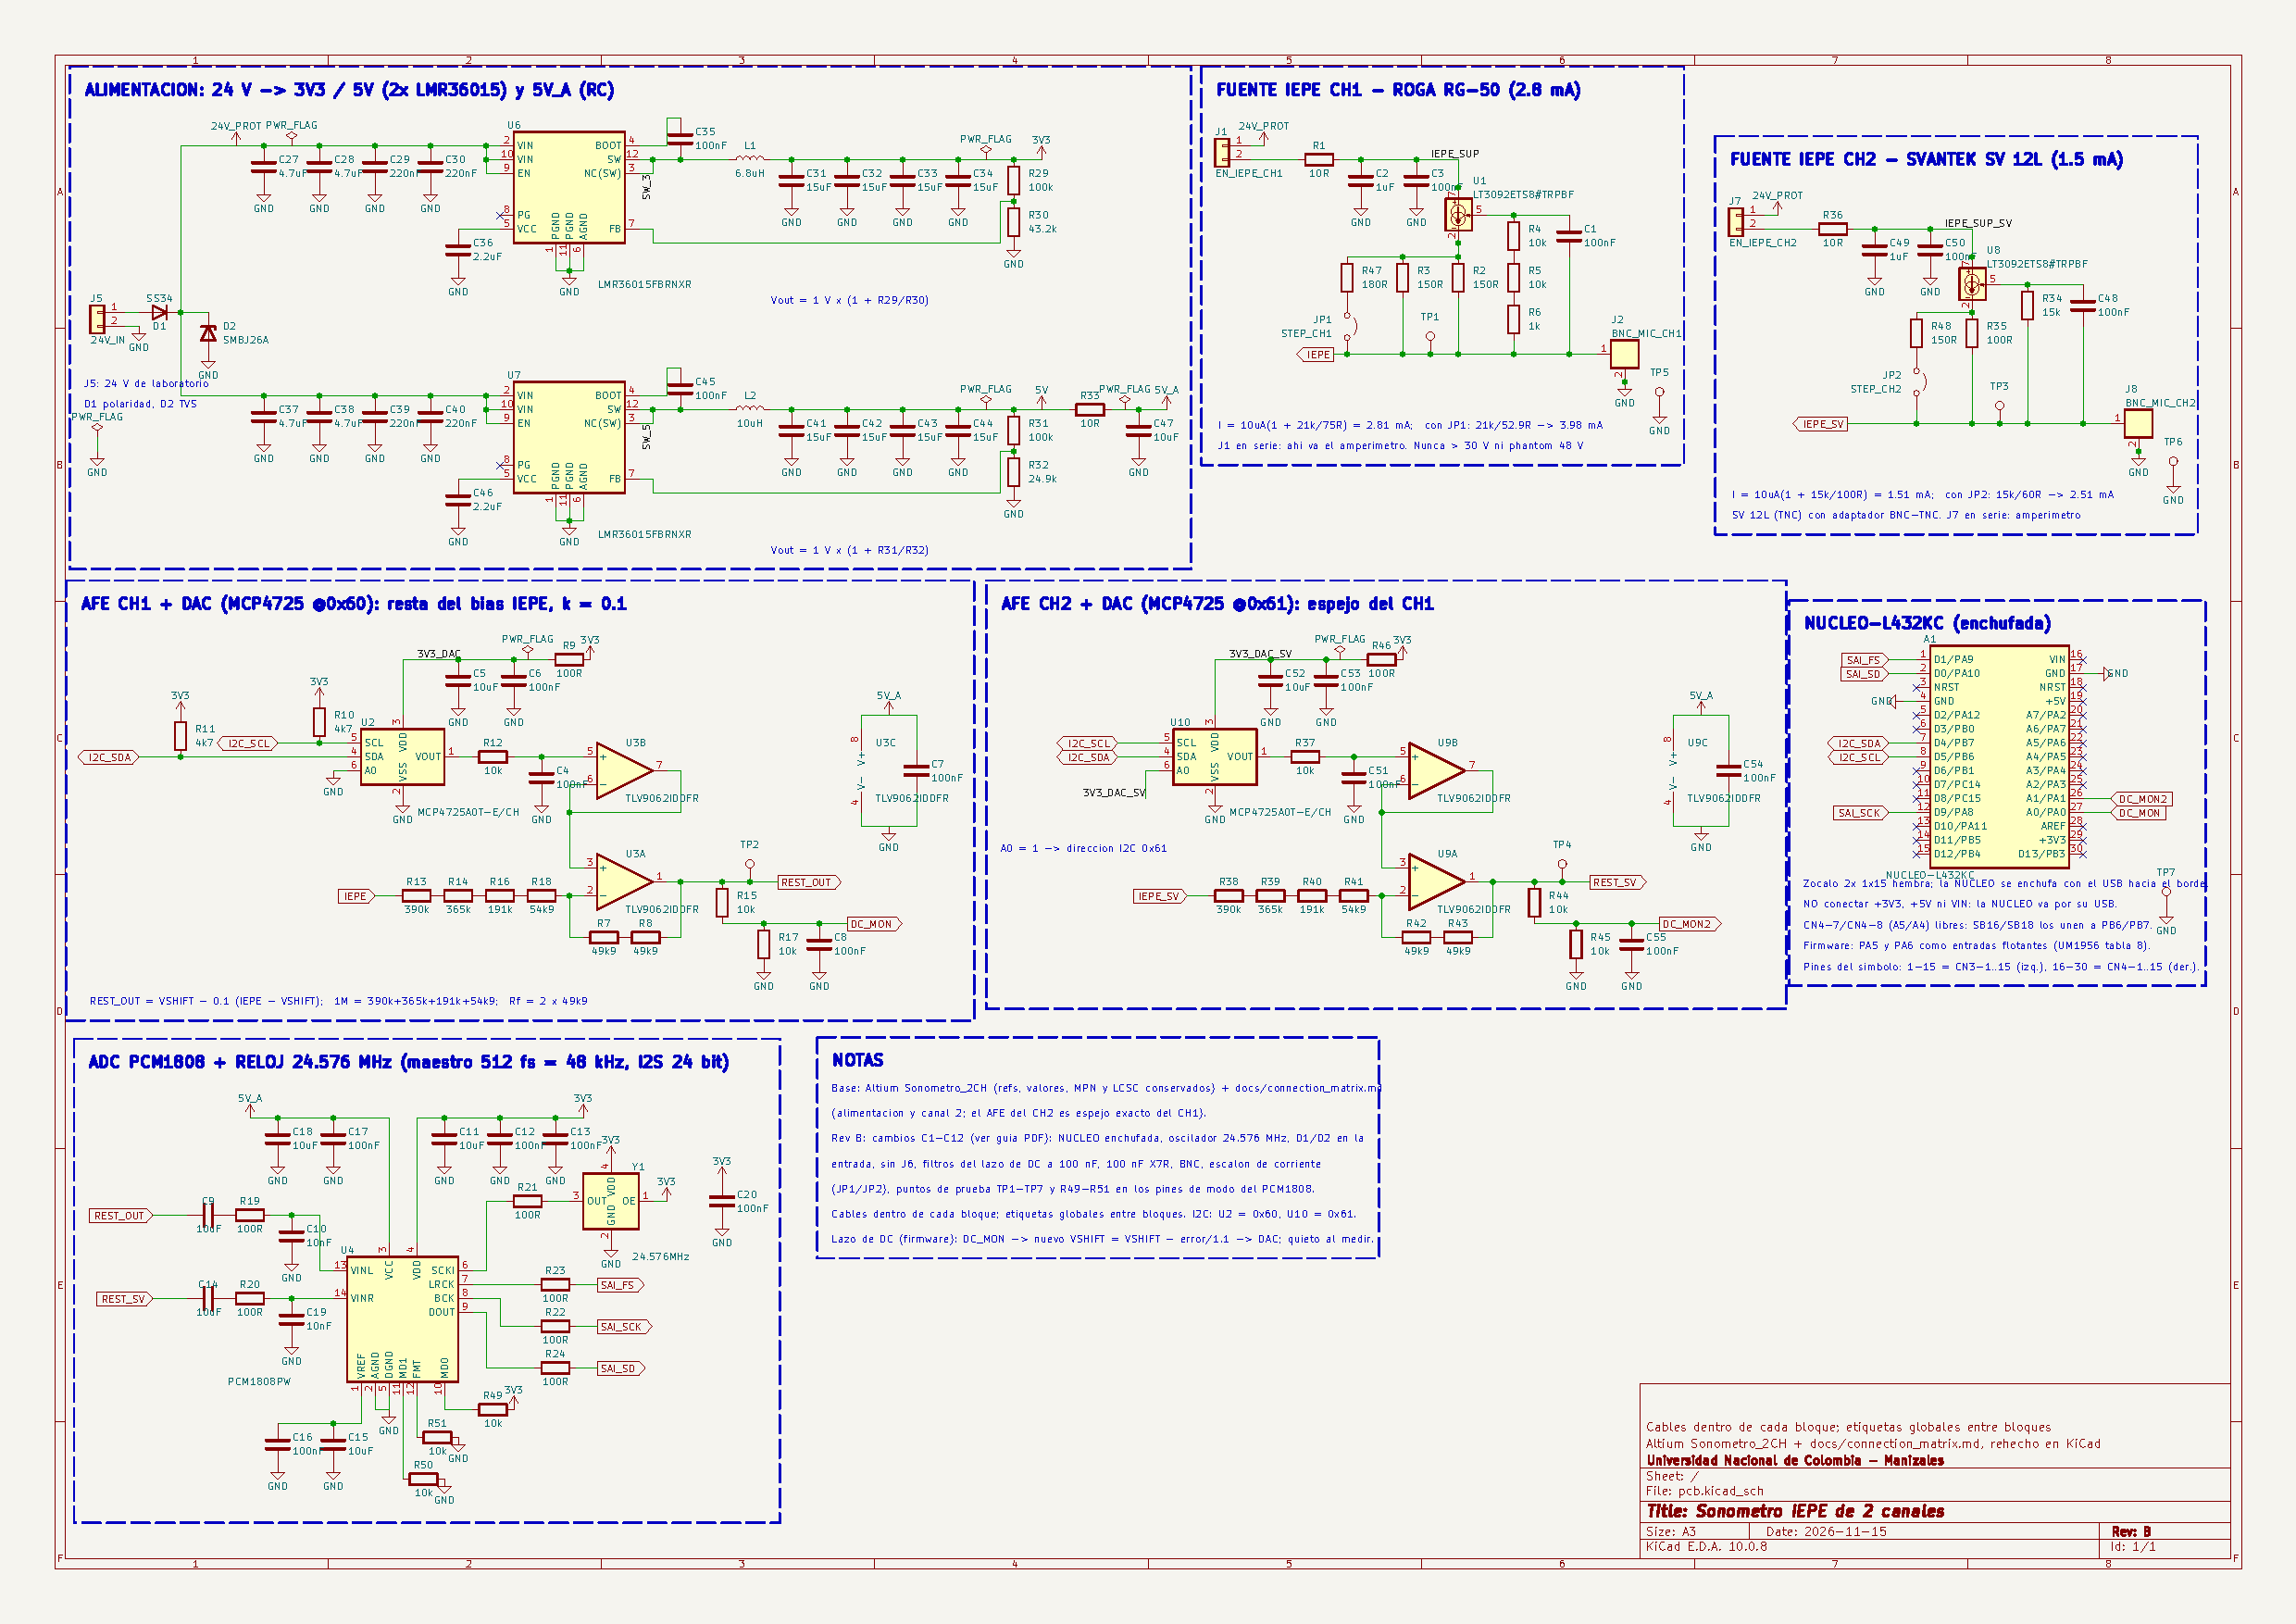
\includepdf[pages=-,fitpaper=true]{esquematico.pdf}
\section{Componentes por bloque}
Columna \emph{Altium}: nombre del componente en la Rocket\_Library que ya usó el equipo (\emph{Gateway} = está
en el proyecto del gateway; \textbf{NUEVO} = hay que crearlo). Un código LCSC con * se encontró en búsqueda web
el 15/11/2026 (confirmar stock al pedir); C55513 es el PCM1808PW\textbf{R} (la versión en carrete, misma pieza).
\emph{Montaje}: JLC = lo monta JLCPCB; Manual = THT que sueldan ustedes (más barato, no paga montaje);
Ninguno = pad de prueba sin componente.
\subsection*{Alimentación: entrada 24 V, buck 3V3, buck 5V y filtro 5V\_A}
{\scriptsize\begin{longtable}{@{}L{0.07\linewidth}L{0.17\linewidth}L{0.17\linewidth}L{0.09\linewidth}L{0.20\linewidth}L{0.14\linewidth}L{0.06\linewidth}@{}}\toprule
\textbf{Ref} & \textbf{Valor} & \textbf{MPN} & \textbf{LCSC} & \textbf{Footprint (KiCad)} & \textbf{Altium} & \textbf{Mont.}\\\midrule\endhead
J5 & 24V\_\allowbreak{}IN & JL126-50002G01 & C394556 & TerminalBlock\_\allowbreak{}MaiXu\_\allowbreak{}MX126-5.0-02P\_\allowbreak{}1x02\_\allowbreak{}P5.00mm & Con\_\allowbreak{}2x1\_\allowbreak{}TH\_\allowbreak{}5mm & Manual\\
D1 & SS34 & SS34 & C8678 & D\_\allowbreak{}SMA & \textbf{NUEVO} & JLC\\
D2 & SMBJ26A & SMBJ26A & C123820 & D\_\allowbreak{}SMB & \textbf{NUEVO} & JLC\\
U6 & LMR36015FBRNXR & LMR36015FBRNXR & C1850339 & Texas\_\allowbreak{}RNX0012A\_\allowbreak{}VQFN-HR-12\_\allowbreak{}2x3mm\_\allowbreak{}P0.5mm & Gateway & JLC\\
L1 & 6.8uH & XAL4030-682MEC &  & L\_\allowbreak{}Coilcraft\_\allowbreak{}XAL4030-XXX & Gateway & JLC\\
C27 & 4.7uF & C5750X7R2A475K230KA &  & C\_\allowbreak{}2220\_\allowbreak{}5750Metric & Gateway & JLC\\
C28 & 4.7uF & C5750X7R2A475K230KA &  & C\_\allowbreak{}2220\_\allowbreak{}5750Metric & Gateway & JLC\\
C29 & 220nF & C0805C224K1RACTU &  & C\_\allowbreak{}0805\_\allowbreak{}2012Metric & Gateway & JLC\\
C30 & 220nF & C0805C224K1RACTU &  & C\_\allowbreak{}0805\_\allowbreak{}2012Metric & Gateway & JLC\\
C31 & 15uF & C3225X7R1C156M250AB &  & C\_\allowbreak{}1210\_\allowbreak{}3225Metric & Gateway & JLC\\
C32 & 15uF & C3225X7R1C156M250AB &  & C\_\allowbreak{}1210\_\allowbreak{}3225Metric & Gateway & JLC\\
C33 & 15uF & C3225X7R1C156M250AB &  & C\_\allowbreak{}1210\_\allowbreak{}3225Metric & Gateway & JLC\\
C34 & 15uF & C3225X7R1C156M250AB &  & C\_\allowbreak{}1210\_\allowbreak{}3225Metric & Gateway & JLC\\
C35 & 100nF & CC0603KRX7R9BB104 & C14663 & C\_\allowbreak{}0603\_\allowbreak{}1608Metric & Cap\_\allowbreak{}0.1uF\_\allowbreak{}0603\_\allowbreak{}50V (cambiar MPN a X7R) & JLC\\
C36 & 2.2uF & C0805C225K5RACTU &  & C\_\allowbreak{}0805\_\allowbreak{}2012Metric & Gateway & JLC\\
R29 & 100k & RC0603FR-07100KL &  & R\_\allowbreak{}0603\_\allowbreak{}1608Metric & Gateway & JLC\\
R30 & 43.2k & RC0603FR-0743K2L &  & R\_\allowbreak{}0603\_\allowbreak{}1608Metric & Gateway & JLC\\
U7 & LMR36015FBRNXR & LMR36015FBRNXR & C1850339 & Texas\_\allowbreak{}RNX0012A\_\allowbreak{}VQFN-HR-12\_\allowbreak{}2x3mm\_\allowbreak{}P0.5mm & Gateway & JLC\\
L2 & 10uH & XAL4040-103MEC &  & L\_\allowbreak{}Coilcraft\_\allowbreak{}XAL4040-XXX & Gateway & JLC\\
C37 & 4.7uF & C5750X7R2A475K230KA &  & C\_\allowbreak{}2220\_\allowbreak{}5750Metric & Gateway & JLC\\
C38 & 4.7uF & C5750X7R2A475K230KA &  & C\_\allowbreak{}2220\_\allowbreak{}5750Metric & Gateway & JLC\\
C39 & 220nF & C0805C224K1RACTU &  & C\_\allowbreak{}0805\_\allowbreak{}2012Metric & Gateway & JLC\\
C40 & 220nF & C0805C224K1RACTU &  & C\_\allowbreak{}0805\_\allowbreak{}2012Metric & Gateway & JLC\\
C41 & 15uF & C3225X7R1C156M250AB &  & C\_\allowbreak{}1210\_\allowbreak{}3225Metric & Gateway & JLC\\
C42 & 15uF & C3225X7R1C156M250AB &  & C\_\allowbreak{}1210\_\allowbreak{}3225Metric & Gateway & JLC\\
C43 & 15uF & C3225X7R1C156M250AB &  & C\_\allowbreak{}1210\_\allowbreak{}3225Metric & Gateway & JLC\\
C44 & 15uF & C3225X7R1C156M250AB &  & C\_\allowbreak{}1210\_\allowbreak{}3225Metric & Gateway & JLC\\
C45 & 100nF & CC0603KRX7R9BB104 & C14663 & C\_\allowbreak{}0603\_\allowbreak{}1608Metric & Cap\_\allowbreak{}0.1uF\_\allowbreak{}0603\_\allowbreak{}50V (cambiar MPN a X7R) & JLC\\
C46 & 2.2uF & C0805C225K5RACTU &  & C\_\allowbreak{}0805\_\allowbreak{}2012Metric & Gateway & JLC\\
R31 & 100k & RC0603FR-07100KL &  & R\_\allowbreak{}0603\_\allowbreak{}1608Metric & Gateway & JLC\\
R32 & 24.9k & RC0603FR-0724K9L &  & R\_\allowbreak{}0603\_\allowbreak{}1608Metric & Gateway & JLC\\
R33 & 10R & CRCW0603010RJNEAHP &  & R\_\allowbreak{}0603\_\allowbreak{}1608Metric & Gateway & JLC\\
C47 & 10uF & TCC0603X5R106K100CT & C380314 & C\_\allowbreak{}0603\_\allowbreak{}1608Metric & Cap\_\allowbreak{}10uF\_\allowbreak{}0603\_\allowbreak{}10V & JLC\\
\bottomrule\end{longtable}}
\subsection*{Fuente IEPE CH1 (ROGA RG-50)}
{\scriptsize\begin{longtable}{@{}L{0.07\linewidth}L{0.17\linewidth}L{0.17\linewidth}L{0.09\linewidth}L{0.20\linewidth}L{0.14\linewidth}L{0.06\linewidth}@{}}\toprule
\textbf{Ref} & \textbf{Valor} & \textbf{MPN} & \textbf{LCSC} & \textbf{Footprint (KiCad)} & \textbf{Altium} & \textbf{Mont.}\\\midrule\endhead
J1 & EN\_\allowbreak{}IEPE\_\allowbreak{}CH1 & JL126-50002G01 & C394556 & TerminalBlock\_\allowbreak{}MaiXu\_\allowbreak{}MX126-5.0-02P\_\allowbreak{}1x02\_\allowbreak{}P5.00mm & Con\_\allowbreak{}2x1\_\allowbreak{}TH\_\allowbreak{}5mm & Manual\\
R1 & 10R & CRCW040210R0FKED &  & R\_\allowbreak{}0402\_\allowbreak{}1005Metric & RES 10 OHM 1\% 1/16W 0402 & JLC\\
C2 & 1uF & CL10A105KB8NNNC & C15849 & C\_\allowbreak{}0603\_\allowbreak{}1608Metric & Cap\_\allowbreak{}1uF\_\allowbreak{}0603\_\allowbreak{}50V & JLC\\
C3 & 100nF & CC0603KRX7R9BB104 & C14663 & C\_\allowbreak{}0603\_\allowbreak{}1608Metric & Cap\_\allowbreak{}0.1uF\_\allowbreak{}0603\_\allowbreak{}50V (cambiar MPN a X7R) & JLC\\
U1 & LT3092ETS8\#TRPBF & LT3092ETS8\#TRPBF & C462641* & TSOT-23-8 & LT3092ETS8TRPBF & JLC\\
R4 & 10k & FRC0603J103TS & C2930027 & R\_\allowbreak{}0603\_\allowbreak{}1608Metric & Res\_\allowbreak{}10k\_\allowbreak{}0603\_\allowbreak{}1/10W & JLC\\
R5 & 10k & FRC0603J103TS & C2930027 & R\_\allowbreak{}0603\_\allowbreak{}1608Metric & Res\_\allowbreak{}10k\_\allowbreak{}0603\_\allowbreak{}1/10W & JLC\\
R6 & 1k & FRC0603J102 TS & C2907113 & R\_\allowbreak{}0603\_\allowbreak{}1608Metric & Res\_\allowbreak{}1k\_\allowbreak{}0603\_\allowbreak{}1/10W & JLC\\
C1 & 100nF & CC0603KRX7R9BB104 & C14663 & C\_\allowbreak{}0603\_\allowbreak{}1608Metric & Cap\_\allowbreak{}0.1uF\_\allowbreak{}0603\_\allowbreak{}50V (cambiar MPN a X7R) & JLC\\
R2 & 150R & RTT031500FTP & C103302 & R\_\allowbreak{}0603\_\allowbreak{}1608Metric & Res\_\allowbreak{}150R\_\allowbreak{}0603\_\allowbreak{}1/10W & JLC\\
R3 & 150R & RTT031500FTP & C103302 & R\_\allowbreak{}0603\_\allowbreak{}1608Metric & Res\_\allowbreak{}150R\_\allowbreak{}0603\_\allowbreak{}1/10W & JLC\\
R47 & 180R & 0603WAF1800T5E & C22828 & R\_\allowbreak{}0603\_\allowbreak{}1608Metric & \textbf{NUEVO} & JLC\\
JP1 & STEP\_\allowbreak{}CH1 & Header 1x2 2.54 + jumper &  & PinHeader\_\allowbreak{}1x02\_\allowbreak{}P2.54mm\_\allowbreak{}Vertical & \textbf{NUEVO} & Manual\\
J2 & BNC\_\allowbreak{}MIC\_\allowbreak{}CH1 & KH-BNC75-3511 & C2837588 & BNC\_\allowbreak{}Kinghelm\_\allowbreak{}KH-BNC75-3511\_\allowbreak{}Horizontal & \textbf{NUEVO} & Manual\\
TP1 & TP\_\allowbreak{}IEPE &  &  & TestPoint\_\allowbreak{}THTPad\_\allowbreak{}D2.0mm\_\allowbreak{}Drill1.0mm & \textbf{NUEVO} & Ninguno\\
TP5 & TP\_\allowbreak{}GND &  &  & TestPoint\_\allowbreak{}THTPad\_\allowbreak{}D2.0mm\_\allowbreak{}Drill1.0mm & \textbf{NUEVO} & Ninguno\\
\bottomrule\end{longtable}}
\subsection*{Fuente IEPE CH2 (Svantek SV 12L)}
{\scriptsize\begin{longtable}{@{}L{0.07\linewidth}L{0.17\linewidth}L{0.17\linewidth}L{0.09\linewidth}L{0.20\linewidth}L{0.14\linewidth}L{0.06\linewidth}@{}}\toprule
\textbf{Ref} & \textbf{Valor} & \textbf{MPN} & \textbf{LCSC} & \textbf{Footprint (KiCad)} & \textbf{Altium} & \textbf{Mont.}\\\midrule\endhead
J7 & EN\_\allowbreak{}IEPE\_\allowbreak{}CH2 & JL126-50002G01 & C394556 & TerminalBlock\_\allowbreak{}MaiXu\_\allowbreak{}MX126-5.0-02P\_\allowbreak{}1x02\_\allowbreak{}P5.00mm & Con\_\allowbreak{}2x1\_\allowbreak{}TH\_\allowbreak{}5mm & Manual\\
R36 & 10R & CRCW040210R0FKED &  & R\_\allowbreak{}0402\_\allowbreak{}1005Metric & RES 10 OHM 1\% 1/16W 0402 & JLC\\
C49 & 1uF & CL10A105KB8NNNC & C15849 & C\_\allowbreak{}0603\_\allowbreak{}1608Metric & Cap\_\allowbreak{}1uF\_\allowbreak{}0603\_\allowbreak{}50V & JLC\\
C50 & 100nF & CC0603KRX7R9BB104 & C14663 & C\_\allowbreak{}0603\_\allowbreak{}1608Metric & Cap\_\allowbreak{}0.1uF\_\allowbreak{}0603\_\allowbreak{}50V (cambiar MPN a X7R) & JLC\\
U8 & LT3092ETS8\#TRPBF & LT3092ETS8\#TRPBF & C462641* & TSOT-23-8 & LT3092ETS8TRPBF & JLC\\
R34 & 15k & RC0603FR-0715KL &  & R\_\allowbreak{}0603\_\allowbreak{}1608Metric & \textbf{NUEVO} & JLC\\
C48 & 100nF & CC0603KRX7R9BB104 & C14663 & C\_\allowbreak{}0603\_\allowbreak{}1608Metric & Cap\_\allowbreak{}0.1uF\_\allowbreak{}0603\_\allowbreak{}50V (cambiar MPN a X7R) & JLC\\
R35 & 100R & RC0603FR-07100RL &  & R\_\allowbreak{}0603\_\allowbreak{}1608Metric & Res\_\allowbreak{}100R\_\allowbreak{}0603\_\allowbreak{}1/10W & JLC\\
R48 & 150R & 0603WAF1500T5E & C22808 & R\_\allowbreak{}0603\_\allowbreak{}1608Metric & Res\_\allowbreak{}150R\_\allowbreak{}0603\_\allowbreak{}1/10W & JLC\\
JP2 & STEP\_\allowbreak{}CH2 & Header 1x2 2.54 + jumper &  & PinHeader\_\allowbreak{}1x02\_\allowbreak{}P2.54mm\_\allowbreak{}Vertical & \textbf{NUEVO} & Manual\\
J8 & BNC\_\allowbreak{}MIC\_\allowbreak{}CH2 & KH-BNC75-3511 & C2837588 & BNC\_\allowbreak{}Kinghelm\_\allowbreak{}KH-BNC75-3511\_\allowbreak{}Horizontal & \textbf{NUEVO} & Manual\\
TP3 & TP\_\allowbreak{}IEPE\_\allowbreak{}SV &  &  & TestPoint\_\allowbreak{}THTPad\_\allowbreak{}D2.0mm\_\allowbreak{}Drill1.0mm & \textbf{NUEVO} & Ninguno\\
TP6 & TP\_\allowbreak{}GND &  &  & TestPoint\_\allowbreak{}THTPad\_\allowbreak{}D2.0mm\_\allowbreak{}Drill1.0mm & \textbf{NUEVO} & Ninguno\\
\bottomrule\end{longtable}}
\subsection*{AFE + DAC CH1}
{\scriptsize\begin{longtable}{@{}L{0.07\linewidth}L{0.17\linewidth}L{0.17\linewidth}L{0.09\linewidth}L{0.20\linewidth}L{0.14\linewidth}L{0.06\linewidth}@{}}\toprule
\textbf{Ref} & \textbf{Valor} & \textbf{MPN} & \textbf{LCSC} & \textbf{Footprint (KiCad)} & \textbf{Altium} & \textbf{Mont.}\\\midrule\endhead
U2 & MCP4725A0T-E/CH & MCP4725A0T-E/CH & C144198* & SOT-23-6 & MCP4725A0T-ECH & JLC\\
U3 & TLV9062IDDFR & TLV9062IDDFR & C2867884* & TSOT-23-8 & TLV9062IDDFR & JLC\\
R7 & 49k9 & RC0603FR-0749K9L & C114624 & R\_\allowbreak{}0603\_\allowbreak{}1608Metric & Res\_\allowbreak{}49k9\_\allowbreak{}0603\_\allowbreak{}1/10W & JLC\\
R8 & 49k9 & RC0603FR-0749K9L & C114624 & R\_\allowbreak{}0603\_\allowbreak{}1608Metric & Res\_\allowbreak{}49k9\_\allowbreak{}0603\_\allowbreak{}1/10W & JLC\\
R9 & 100R & FRC0603J101 TS & C2907089 & R\_\allowbreak{}0603\_\allowbreak{}1608Metric & Res\_\allowbreak{}100R\_\allowbreak{}0603\_\allowbreak{}1/10W & JLC\\
R10 & 4k7 & SCR0603F4K7 & C3016318 & R\_\allowbreak{}0603\_\allowbreak{}1608Metric & Res\_\allowbreak{}4k7\_\allowbreak{}0603\_\allowbreak{}1/10W & JLC\\
R11 & 4k7 & SCR0603F4K7 & C3016318 & R\_\allowbreak{}0603\_\allowbreak{}1608Metric & Res\_\allowbreak{}4k7\_\allowbreak{}0603\_\allowbreak{}1/10W & JLC\\
R12 & 10k & FRC0603J103TS & C2930027 & R\_\allowbreak{}0603\_\allowbreak{}1608Metric & Res\_\allowbreak{}10k\_\allowbreak{}0603\_\allowbreak{}1/10W & JLC\\
R13 & 390k & RC0603FR-07390KL & C137735 & R\_\allowbreak{}0603\_\allowbreak{}1608Metric & Res\_\allowbreak{}390k\_\allowbreak{}0603\_\allowbreak{}1/10W & JLC\\
R14 & 365k & RC0603FR-07365KL & C185336 & R\_\allowbreak{}0603\_\allowbreak{}1608Metric & Res\_\allowbreak{}365k\_\allowbreak{}0603\_\allowbreak{}1/10W & JLC\\
R15 & 10k & FRC0603J103TS & C2930027 & R\_\allowbreak{}0603\_\allowbreak{}1608Metric & Res\_\allowbreak{}10k\_\allowbreak{}0603\_\allowbreak{}1/10W & JLC\\
R16 & 191k & AC0603FR-07191KL & C227635 & R\_\allowbreak{}0603\_\allowbreak{}1608Metric & Res\_\allowbreak{}191k\_\allowbreak{}0603\_\allowbreak{}1/10W & JLC\\
R17 & 10k & FRC0603J103TS & C2930027 & R\_\allowbreak{}0603\_\allowbreak{}1608Metric & Res\_\allowbreak{}10k\_\allowbreak{}0603\_\allowbreak{}1/10W & JLC\\
R18 & 54k9 & RC0603FR-0754K9L & C185321 & R\_\allowbreak{}0603\_\allowbreak{}1608Metric & Res\_\allowbreak{}54k9\_\allowbreak{}0603\_\allowbreak{}1/10W & JLC\\
C4 & 100nF & CC0603KRX7R9BB104 & C14663 & C\_\allowbreak{}0603\_\allowbreak{}1608Metric & Cap\_\allowbreak{}0.1uF\_\allowbreak{}0603\_\allowbreak{}50V (cambiar MPN a X7R) & JLC\\
C5 & 10uF & TCC0603X5R106K100CT & C380314 & C\_\allowbreak{}0603\_\allowbreak{}1608Metric & Cap\_\allowbreak{}10uF\_\allowbreak{}0603\_\allowbreak{}10V & JLC\\
C6 & 100nF & CC0603KRX7R9BB104 & C14663 & C\_\allowbreak{}0603\_\allowbreak{}1608Metric & Cap\_\allowbreak{}0.1uF\_\allowbreak{}0603\_\allowbreak{}50V (cambiar MPN a X7R) & JLC\\
C7 & 100nF & CC0603KRX7R9BB104 & C14663 & C\_\allowbreak{}0603\_\allowbreak{}1608Metric & Cap\_\allowbreak{}0.1uF\_\allowbreak{}0603\_\allowbreak{}50V (cambiar MPN a X7R) & JLC\\
C8 & 100nF & CC0603KRX7R9BB104 & C14663 & C\_\allowbreak{}0603\_\allowbreak{}1608Metric & Cap\_\allowbreak{}0.1uF\_\allowbreak{}0603\_\allowbreak{}50V (cambiar MPN a X7R) & JLC\\
TP2 & TP\_\allowbreak{}REST\_\allowbreak{}OUT &  &  & TestPoint\_\allowbreak{}THTPad\_\allowbreak{}D2.0mm\_\allowbreak{}Drill1.0mm & \textbf{NUEVO} & Ninguno\\
\bottomrule\end{longtable}}
\subsection*{AFE + DAC CH2}
{\scriptsize\begin{longtable}{@{}L{0.07\linewidth}L{0.17\linewidth}L{0.17\linewidth}L{0.09\linewidth}L{0.20\linewidth}L{0.14\linewidth}L{0.06\linewidth}@{}}\toprule
\textbf{Ref} & \textbf{Valor} & \textbf{MPN} & \textbf{LCSC} & \textbf{Footprint (KiCad)} & \textbf{Altium} & \textbf{Mont.}\\\midrule\endhead
U9 & TLV9062IDDFR & TLV9062IDDFR & C2867884* & TSOT-23-8 & TLV9062IDDFR & JLC\\
U10 & MCP4725A0T-E/CH & MCP4725A0T-E/CH & C144198* & SOT-23-6 & MCP4725A0T-ECH & JLC\\
R37 & 10k & FRC0603J103TS & C2930027 & R\_\allowbreak{}0603\_\allowbreak{}1608Metric & Res\_\allowbreak{}10k\_\allowbreak{}0603\_\allowbreak{}1/10W & JLC\\
R38 & 390k & RC0603FR-07390KL & C137735 & R\_\allowbreak{}0603\_\allowbreak{}1608Metric & Res\_\allowbreak{}390k\_\allowbreak{}0603\_\allowbreak{}1/10W & JLC\\
R39 & 365k & RC0603FR-07365KL & C185336 & R\_\allowbreak{}0603\_\allowbreak{}1608Metric & Res\_\allowbreak{}365k\_\allowbreak{}0603\_\allowbreak{}1/10W & JLC\\
R40 & 191k & AC0603FR-07191KL & C227635 & R\_\allowbreak{}0603\_\allowbreak{}1608Metric & Res\_\allowbreak{}191k\_\allowbreak{}0603\_\allowbreak{}1/10W & JLC\\
R41 & 54k9 & RC0603FR-0754K9L & C185321 & R\_\allowbreak{}0603\_\allowbreak{}1608Metric & Res\_\allowbreak{}54k9\_\allowbreak{}0603\_\allowbreak{}1/10W & JLC\\
R42 & 49k9 & RC0603FR-0749K9L & C114624 & R\_\allowbreak{}0603\_\allowbreak{}1608Metric & Res\_\allowbreak{}49k9\_\allowbreak{}0603\_\allowbreak{}1/10W & JLC\\
R43 & 49k9 & RC0603FR-0749K9L & C114624 & R\_\allowbreak{}0603\_\allowbreak{}1608Metric & Res\_\allowbreak{}49k9\_\allowbreak{}0603\_\allowbreak{}1/10W & JLC\\
R44 & 10k & FRC0603J103TS & C2930027 & R\_\allowbreak{}0603\_\allowbreak{}1608Metric & Res\_\allowbreak{}10k\_\allowbreak{}0603\_\allowbreak{}1/10W & JLC\\
R45 & 10k & FRC0603J103TS & C2930027 & R\_\allowbreak{}0603\_\allowbreak{}1608Metric & Res\_\allowbreak{}10k\_\allowbreak{}0603\_\allowbreak{}1/10W & JLC\\
R46 & 100R & FRC0603J101 TS & C2907089 & R\_\allowbreak{}0603\_\allowbreak{}1608Metric & Res\_\allowbreak{}100R\_\allowbreak{}0603\_\allowbreak{}1/10W & JLC\\
C51 & 100nF & CC0603KRX7R9BB104 & C14663 & C\_\allowbreak{}0603\_\allowbreak{}1608Metric & Cap\_\allowbreak{}0.1uF\_\allowbreak{}0603\_\allowbreak{}50V (cambiar MPN a X7R) & JLC\\
C52 & 10uF & TCC0603X5R106K100CT & C380314 & C\_\allowbreak{}0603\_\allowbreak{}1608Metric & Cap\_\allowbreak{}10uF\_\allowbreak{}0603\_\allowbreak{}10V & JLC\\
C53 & 100nF & CC0603KRX7R9BB104 & C14663 & C\_\allowbreak{}0603\_\allowbreak{}1608Metric & Cap\_\allowbreak{}0.1uF\_\allowbreak{}0603\_\allowbreak{}50V (cambiar MPN a X7R) & JLC\\
C54 & 100nF & CC0603KRX7R9BB104 & C14663 & C\_\allowbreak{}0603\_\allowbreak{}1608Metric & Cap\_\allowbreak{}0.1uF\_\allowbreak{}0603\_\allowbreak{}50V (cambiar MPN a X7R) & JLC\\
C55 & 100nF & CC0603KRX7R9BB104 & C14663 & C\_\allowbreak{}0603\_\allowbreak{}1608Metric & Cap\_\allowbreak{}0.1uF\_\allowbreak{}0603\_\allowbreak{}50V (cambiar MPN a X7R) & JLC\\
TP4 & TP\_\allowbreak{}REST\_\allowbreak{}SV &  &  & TestPoint\_\allowbreak{}THTPad\_\allowbreak{}D2.0mm\_\allowbreak{}Drill1.0mm & \textbf{NUEVO} & Ninguno\\
\bottomrule\end{longtable}}
\subsection*{ADC PCM1808 + reloj}
{\scriptsize\begin{longtable}{@{}L{0.07\linewidth}L{0.17\linewidth}L{0.17\linewidth}L{0.09\linewidth}L{0.20\linewidth}L{0.14\linewidth}L{0.06\linewidth}@{}}\toprule
\textbf{Ref} & \textbf{Valor} & \textbf{MPN} & \textbf{LCSC} & \textbf{Footprint (KiCad)} & \textbf{Altium} & \textbf{Mont.}\\\midrule\endhead
U4 & PCM1808PW & PCM1808PW & C55513* & TSSOP-14\_\allowbreak{}4.4x5mm\_\allowbreak{}P0.65mm & PCM1808PW & JLC\\
Y1 & 24.576MHz & O322524576MEEA4SC & C27869 & Oscillator\_\allowbreak{}YXC\_\allowbreak{}SMD3225-4Pin\_\allowbreak{}3.2x2.5mm & \textbf{NUEVO} & JLC\\
C9 & 10uF & TCC0603X5R106K100CT & C380314 & C\_\allowbreak{}0603\_\allowbreak{}1608Metric & Cap\_\allowbreak{}10uF\_\allowbreak{}0603\_\allowbreak{}10V & JLC\\
C10 & 10nF & C0402C103K3REC7411 &  & C\_\allowbreak{}0402\_\allowbreak{}1005Metric & Cap\_\allowbreak{}10nF\_\allowbreak{}0402\_\allowbreak{}25V & JLC\\
C11 & 10uF & TCC0603X5R106K100CT & C380314 & C\_\allowbreak{}0603\_\allowbreak{}1608Metric & Cap\_\allowbreak{}10uF\_\allowbreak{}0603\_\allowbreak{}10V & JLC\\
C12 & 100nF & CC0603KRX7R9BB104 & C14663 & C\_\allowbreak{}0603\_\allowbreak{}1608Metric & Cap\_\allowbreak{}0.1uF\_\allowbreak{}0603\_\allowbreak{}50V (cambiar MPN a X7R) & JLC\\
C13 & 100nF & CC0603KRX7R9BB104 & C14663 & C\_\allowbreak{}0603\_\allowbreak{}1608Metric & Cap\_\allowbreak{}0.1uF\_\allowbreak{}0603\_\allowbreak{}50V (cambiar MPN a X7R) & JLC\\
C14 & 10uF & TCC0603X5R106K100CT & C380314 & C\_\allowbreak{}0603\_\allowbreak{}1608Metric & Cap\_\allowbreak{}10uF\_\allowbreak{}0603\_\allowbreak{}10V & JLC\\
C15 & 10uF & TCC0603X5R106K100CT & C380314 & C\_\allowbreak{}0603\_\allowbreak{}1608Metric & Cap\_\allowbreak{}10uF\_\allowbreak{}0603\_\allowbreak{}10V & JLC\\
C16 & 100nF & CC0603KRX7R9BB104 & C14663 & C\_\allowbreak{}0603\_\allowbreak{}1608Metric & Cap\_\allowbreak{}0.1uF\_\allowbreak{}0603\_\allowbreak{}50V (cambiar MPN a X7R) & JLC\\
C17 & 100nF & CC0603KRX7R9BB104 & C14663 & C\_\allowbreak{}0603\_\allowbreak{}1608Metric & Cap\_\allowbreak{}0.1uF\_\allowbreak{}0603\_\allowbreak{}50V (cambiar MPN a X7R) & JLC\\
C18 & 10uF & TCC0603X5R106K100CT & C380314 & C\_\allowbreak{}0603\_\allowbreak{}1608Metric & Cap\_\allowbreak{}10uF\_\allowbreak{}0603\_\allowbreak{}10V & JLC\\
C19 & 10nF & C0402C103K3REC7411 &  & C\_\allowbreak{}0402\_\allowbreak{}1005Metric & Cap\_\allowbreak{}10nF\_\allowbreak{}0402\_\allowbreak{}25V & JLC\\
C20 & 100nF & CC0603KRX7R9BB104 & C14663 & C\_\allowbreak{}0603\_\allowbreak{}1608Metric & Cap\_\allowbreak{}0.1uF\_\allowbreak{}0603\_\allowbreak{}50V (cambiar MPN a X7R) & JLC\\
R19 & 100R & FRC0603J101 TS & C2907089 & R\_\allowbreak{}0603\_\allowbreak{}1608Metric & Res\_\allowbreak{}100R\_\allowbreak{}0603\_\allowbreak{}1/10W & JLC\\
R20 & 100R & FRC0603J101 TS & C2907089 & R\_\allowbreak{}0603\_\allowbreak{}1608Metric & Res\_\allowbreak{}100R\_\allowbreak{}0603\_\allowbreak{}1/10W & JLC\\
R21 & 100R & FRC0603J101 TS & C2907089 & R\_\allowbreak{}0603\_\allowbreak{}1608Metric & Res\_\allowbreak{}100R\_\allowbreak{}0603\_\allowbreak{}1/10W & JLC\\
R22 & 100R & FRC0603J101 TS & C2907089 & R\_\allowbreak{}0603\_\allowbreak{}1608Metric & Res\_\allowbreak{}100R\_\allowbreak{}0603\_\allowbreak{}1/10W & JLC\\
R23 & 100R & FRC0603J101 TS & C2907089 & R\_\allowbreak{}0603\_\allowbreak{}1608Metric & Res\_\allowbreak{}100R\_\allowbreak{}0603\_\allowbreak{}1/10W & JLC\\
R24 & 100R & FRC0603J101 TS & C2907089 & R\_\allowbreak{}0603\_\allowbreak{}1608Metric & Res\_\allowbreak{}100R\_\allowbreak{}0603\_\allowbreak{}1/10W & JLC\\
R49 & 10k & FRC0603J103TS & C2930027 & R\_\allowbreak{}0603\_\allowbreak{}1608Metric & Res\_\allowbreak{}10k\_\allowbreak{}0603\_\allowbreak{}1/10W & JLC\\
R50 & 10k & FRC0603J103TS & C2930027 & R\_\allowbreak{}0603\_\allowbreak{}1608Metric & Res\_\allowbreak{}10k\_\allowbreak{}0603\_\allowbreak{}1/10W & JLC\\
R51 & 10k & FRC0603J103TS & C2930027 & R\_\allowbreak{}0603\_\allowbreak{}1608Metric & Res\_\allowbreak{}10k\_\allowbreak{}0603\_\allowbreak{}1/10W & JLC\\
TP7 & TP\_\allowbreak{}GND &  &  & TestPoint\_\allowbreak{}THTPad\_\allowbreak{}D2.0mm\_\allowbreak{}Drill1.0mm & \textbf{NUEVO} & Ninguno\\
\bottomrule\end{longtable}}
\subsection*{NUCLEO-L432KC (zócalo)}
{\scriptsize\begin{longtable}{@{}L{0.07\linewidth}L{0.17\linewidth}L{0.17\linewidth}L{0.09\linewidth}L{0.20\linewidth}L{0.14\linewidth}L{0.06\linewidth}@{}}\toprule
\textbf{Ref} & \textbf{Valor} & \textbf{MPN} & \textbf{LCSC} & \textbf{Footprint (KiCad)} & \textbf{Altium} & \textbf{Mont.}\\\midrule\endhead
A1 & NUCLEO-L432KC & KH-2.54FH-1X15P-H8.5 (x2) + NUCLEO-L432KC & C2932676 (x2) & NUCLEO-32\_\allowbreak{}Socket\_\allowbreak{}2x15\_\allowbreak{}P2.54mm\_\allowbreak{}Row15.24mm & \textbf{NUEVO} & Manual\\
\bottomrule\end{longtable}}
\subsection*{Lista de compra consolidada}
{\scriptsize\begin{longtable}{@{}L{0.05\linewidth}L{0.17\linewidth}L{0.2\linewidth}L{0.1\linewidth}L{0.07\linewidth}L{0.34\linewidth}@{}}\toprule
\textbf{Cant.} & \textbf{Valor} & \textbf{MPN} & \textbf{LCSC} & \textbf{Mont.} & \textbf{Referencias}\\\midrule\endhead
1 & 24V\_\allowbreak{}IN & JL126-50002G01 & C394556 & Manual & J5\\
1 & SS34 & SS34 & C8678 & JLC & D1\\
1 & SMBJ26A & SMBJ26A & C123820 & JLC & D2\\
2 & LMR36015FBRNXR & LMR36015FBRNXR & C1850339 & JLC & U6, U7\\
1 & 6.8uH & XAL4030-682MEC &  & JLC & L1\\
4 & 4.7uF & C5750X7R2A475K230KA &  & JLC & C27, C28, C37, C38\\
4 & 220nF & C0805C224K1RACTU &  & JLC & C29, C30, C39, C40\\
8 & 15uF & C3225X7R1C156M250AB &  & JLC & C31, C32, C33, C34, C41, C42, C43, C44\\
19 & 100nF & CC0603KRX7R9BB104 & C14663 & JLC & C35, C45, C3, C1, C50, C48, C4, C6, C7, C8, C51, C53, C54, C55, C12, C13, C16, C17, C20\\
2 & 2.2uF & C0805C225K5RACTU &  & JLC & C36, C46\\
2 & 100k & RC0603FR-07100KL &  & JLC & R29, R31\\
1 & 43.2k & RC0603FR-0743K2L &  & JLC & R30\\
1 & 10uH & XAL4040-103MEC &  & JLC & L2\\
1 & 24.9k & RC0603FR-0724K9L &  & JLC & R32\\
1 & 10R & CRCW0603010RJNEAHP &  & JLC & R33\\
8 & 10uF & TCC0603X5R106K100CT & C380314 & JLC & C47, C5, C52, C9, C11, C14, C15, C18\\
1 & EN\_\allowbreak{}IEPE\_\allowbreak{}CH1 & JL126-50002G01 & C394556 & Manual & J1\\
2 & 10R & CRCW040210R0FKED &  & JLC & R1, R36\\
2 & 1uF & CL10A105KB8NNNC & C15849 & JLC & C2, C49\\
2 & LT3092ETS8\#TRPBF & LT3092ETS8\#TRPBF & C462641* & JLC & U1, U8\\
11 & 10k & FRC0603J103TS & C2930027 & JLC & R4, R5, R12, R15, R17, R37, R44, R45, R49, R50, R51\\
1 & 1k & FRC0603J102 TS & C2907113 & JLC & R6\\
2 & 150R & RTT031500FTP & C103302 & JLC & R2, R3\\
1 & 180R & 0603WAF1800T5E & C22828 & JLC & R47\\
1 & STEP\_\allowbreak{}CH1 & Header 1x2 2.54 + jumper &  & Manual & JP1\\
1 & BNC\_\allowbreak{}MIC\_\allowbreak{}CH1 & KH-BNC75-3511 & C2837588 & Manual & J2\\
1 & EN\_\allowbreak{}IEPE\_\allowbreak{}CH2 & JL126-50002G01 & C394556 & Manual & J7\\
1 & 15k & RC0603FR-0715KL &  & JLC & R34\\
1 & 100R & RC0603FR-07100RL &  & JLC & R35\\
1 & 150R & 0603WAF1500T5E & C22808 & JLC & R48\\
1 & STEP\_\allowbreak{}CH2 & Header 1x2 2.54 + jumper &  & Manual & JP2\\
1 & BNC\_\allowbreak{}MIC\_\allowbreak{}CH2 & KH-BNC75-3511 & C2837588 & Manual & J8\\
2 & MCP4725A0T-E/CH & MCP4725A0T-E/CH & C144198* & JLC & U2, U10\\
2 & TLV9062IDDFR & TLV9062IDDFR & C2867884* & JLC & U3, U9\\
4 & 49k9 & RC0603FR-0749K9L & C114624 & JLC & R7, R8, R42, R43\\
8 & 100R & FRC0603J101 TS & C2907089 & JLC & R9, R46, R19, R20, R21, R22, R23, R24\\
2 & 4k7 & SCR0603F4K7 & C3016318 & JLC & R10, R11\\
2 & 390k & RC0603FR-07390KL & C137735 & JLC & R13, R38\\
2 & 365k & RC0603FR-07365KL & C185336 & JLC & R14, R39\\
2 & 191k & AC0603FR-07191KL & C227635 & JLC & R16, R40\\
2 & 54k9 & RC0603FR-0754K9L & C185321 & JLC & R18, R41\\
1 & PCM1808PW & PCM1808PW & C55513* & JLC & U4\\
1 & 24.576MHz & O322524576MEEA4SC & C27869 & JLC & Y1\\
2 & 10nF & C0402C103K3REC7411 &  & JLC & C10, C19\\
1 & NUCLEO-L432KC & KH-2.54FH-1X15P-H8.5 (x2) + NUCLEO-L432KC & C2932676 (x2) & Manual & A1\\
\bottomrule\end{longtable}}
Además, fuera de la placa: un \textbf{adaptador BNC macho a TNC hembra} para el SV 12L, dos
\textbf{jumpers} de 2.54 mm (JP1, JP2) y la \textbf{NUCLEO-L432KC}.
\section{Conexiones red por red}
Cada fila es una red: todos los pines listados deben quedar unidos (con cable o con la misma
etiqueta/puerto). Formato \texttt{Ref.pin(nombre)}. Las redes sin etiqueta en el esquemático aparecen con
un nombre descriptivo entre corchetes (no hace falta ponerles etiqueta en Altium).
\subsection*{Alimentación: entrada 24 V, buck 3V3, buck 5V y filtro 5V\_A}
{\footnotesize\begin{longtable}{@{}L{0.2\linewidth}L{0.06\linewidth}L{0.7\linewidth}@{}}\toprule
\textbf{Red} & \textbf{Pines} & \textbf{Conexiones}\\\midrule\endhead
24V\_\allowbreak{}PROT & 18 & D1.1(K), D2.1(K), U6.2(VIN), U6.9(EN), U6.10(VIN), C27.1, C28.1, C29.1, C30.1, U7.2(VIN), U7.9(EN), U7.10(VIN), C37.1, C38.1, C39.1, C40.1, J1.1(Pin\_\allowbreak{}1), J7.1(Pin\_\allowbreak{}1)\\
3V3 & 18 & L1.2, C31.1, C32.1, C33.1, C34.1, R29.1, R9.2, R10.2, R11.2, R46.2, U4.4(VDD), Y1.1(OE), Y1.4(VDD), C11.1, C12.1, C13.1, C20.1, R49.1\\
5V & 7 & L2.2, C41.1, C42.1, C43.1, C44.1, R31.1, R33.1\\
5V\_\allowbreak{}A & 9 & R33.2, C47.1, U3.8(V+), C7.2, U9.8(V+), C54.2, U4.3(VCC), C17.1, C18.1\\
GND & 76 & J5.2(Pin\_\allowbreak{}2), D2.2(A), U6.1(PGND), U6.6(AGND), U6.11(PGND), C27.2, C28.2, C29.2, C30.2, C31.2, C32.2, C33.2, C34.2, C36.2, R30.2, U7.1(PGND), U7.6(AGND), U7.11(PGND), C37.2, C38.2, C39.2, C40.2, C41.2, C42.2, C43.2, C44.2, C46.2, R32.2, C47.2, C2.2, C3.2, J2.2(SHIELD), J2.3(SHIELD), J2.4(SHIELD), TP5.1, C49.2, C50.2, J8.2(SHIELD), J8.3(SHIELD), J8.4(SHIELD), TP6.1, U2.2(VSS), U2.6(A0), U3.4(V-), R17.1, C4.2, C5.2, C6.2, C7.1, C8.2, U9.4(V-), U10.2(VSS), R45.1, C51.2, C52.2, C53.2, C54.1, C55.2, U4.2(AGND), U4.5(DGND), Y1.2(GND), C10.2, C11.2, C12.2, C13.2, C15.2, C16.2, C17.2, C18.2, C19.2, C20.2, R50.2, R51.2, TP7.1, A1.4(GND), A1.17(GND)\\
SW\_\allowbreak{}3 & 4 & U6.3(NC(SW)), U6.12(SW), L1.1, C35.2\\
SW\_\allowbreak{}5 & 4 & U7.3(NC(SW)), U7.12(SW), L2.1, C45.2\\
{[}24V\_\allowbreak{}IN{]} & 2 & J5.1(Pin\_\allowbreak{}1), D1.2(A)\\
{[}BOOT\_\allowbreak{}3{]} & 2 & U6.4(BOOT), C35.1\\
{[}BOOT\_\allowbreak{}5{]} & 2 & U7.4(BOOT), C45.1\\
{[}FB\_\allowbreak{}3{]} & 3 & U6.7(FB), R29.2, R30.1\\
{[}FB\_\allowbreak{}5{]} & 3 & U7.7(FB), R31.2, R32.1\\
{[}VCC\_\allowbreak{}3{]} & 2 & U6.5(VCC), C36.1\\
{[}VCC\_\allowbreak{}5{]} & 2 & U7.5(VCC), C46.1\\
\bottomrule\end{longtable}}
\subsection*{Fuente IEPE CH1 (ROGA RG-50)}
{\footnotesize\begin{longtable}{@{}L{0.2\linewidth}L{0.06\linewidth}L{0.7\linewidth}@{}}\toprule
\textbf{Red} & \textbf{Pines} & \textbf{Conexiones}\\\midrule\endhead
IEPE & 8 & R6.2, C1.2, R2.1, R3.1, JP1.2(B), J2.1(SIG), TP1.1, R13.2\\
IEPE\_\allowbreak{}SUP & 5 & R1.2, C2.1, C3.1, U1.7(IN), U1.8(IN)\\
{[}IEPE\_\allowbreak{}FEED{]} & 2 & J1.2(Pin\_\allowbreak{}2), R1.1\\
{[}OUT\_\allowbreak{}I{]} & 6 & U1.2(OUT), U1.3(OUT), U1.4(OUT), R2.2, R3.2, R47.1\\
{[}SET\_\allowbreak{}I{]} & 3 & U1.5(SET), R4.2, C1.1\\
{[}SET\_\allowbreak{}MID{]} & 2 & R4.1, R5.2\\
{[}SET\_\allowbreak{}MID2{]} & 2 & R5.1, R6.1\\
{[}STEP1{]} & 2 & R47.2, JP1.1(A)\\
\bottomrule\end{longtable}}
\subsection*{Fuente IEPE CH2 (Svantek SV 12L)}
{\footnotesize\begin{longtable}{@{}L{0.2\linewidth}L{0.06\linewidth}L{0.7\linewidth}@{}}\toprule
\textbf{Red} & \textbf{Pines} & \textbf{Conexiones}\\\midrule\endhead
IEPE\_\allowbreak{}SUP\_\allowbreak{}SV & 5 & R36.2, C49.1, C50.1, U8.7(IN), U8.8(IN)\\
IEPE\_\allowbreak{}SV & 7 & R34.2, C48.2, R35.2, JP2.2(B), J8.1(SIG), TP3.1, R38.2\\
{[}IEPE\_\allowbreak{}FEED\_\allowbreak{}SV{]} & 2 & J7.2(Pin\_\allowbreak{}2), R36.1\\
{[}OUT\_\allowbreak{}SV{]} & 5 & U8.2(OUT), U8.3(OUT), U8.4(OUT), R35.1, R48.1\\
{[}SET\_\allowbreak{}SV{]} & 3 & U8.5(SET), R34.1, C48.1\\
{[}STEP2{]} & 2 & R48.2, JP2.1(A)\\
\bottomrule\end{longtable}}
\subsection*{AFE + DAC CH1}
{\footnotesize\begin{longtable}{@{}L{0.2\linewidth}L{0.06\linewidth}L{0.7\linewidth}@{}}\toprule
\textbf{Red} & \textbf{Pines} & \textbf{Conexiones}\\\midrule\endhead
3V3\_\allowbreak{}DAC & 4 & U2.3(VDD), R9.1, C5.1, C6.1\\
DC\_\allowbreak{}MON & 4 & R15.1, R17.2, C8.1, A1.27(A0/PA0)\\
I2C\_\allowbreak{}SCL & 4 & U2.5(SCL), R10.1, U10.5(SCL), A1.8(D5/PB6)\\
I2C\_\allowbreak{}SDA & 4 & U2.4(SDA), R11.1, U10.4(SDA), A1.7(D4/PB7)\\
REST\_\allowbreak{}OUT & 5 & U3.1, R8.1, R15.2, TP2.1, C9.1\\
{[}DAC\_\allowbreak{}F{]} & 3 & U3.5(+), R12.2, C4.1\\
{[}DAC\_\allowbreak{}RAW{]} & 2 & U2.1(VOUT), R12.1\\
{[}FB\_\allowbreak{}MID{]} & 2 & R7.2, R8.2\\
{[}IEPE\_\allowbreak{}DIV1{]} & 2 & R13.1, R14.2\\
{[}IEPE\_\allowbreak{}DIV2{]} & 2 & R14.1, R16.2\\
{[}IEPE\_\allowbreak{}DIV3{]} & 2 & R16.1, R18.2\\
{[}SUM{]} & 3 & U3.2(-), R7.1, R18.1\\
{[}VSHIFT{]} & 3 & U3.3(+), U3.6(-), U3.7\\
\bottomrule\end{longtable}}
\subsection*{AFE + DAC CH2}
{\footnotesize\begin{longtable}{@{}L{0.2\linewidth}L{0.06\linewidth}L{0.7\linewidth}@{}}\toprule
\textbf{Red} & \textbf{Pines} & \textbf{Conexiones}\\\midrule\endhead
3V3\_\allowbreak{}DAC\_\allowbreak{}SV & 5 & U10.3(VDD), U10.6(A0), R46.1, C52.1, C53.1\\
DC\_\allowbreak{}MON2 & 4 & R44.1, R45.2, C55.1, A1.26(A1/PA1)\\
REST\_\allowbreak{}SV & 5 & U9.1, R43.1, R44.2, TP4.1, C14.1\\
{[}DAC\_\allowbreak{}F\_\allowbreak{}SV{]} & 3 & U9.5(+), R37.2, C51.1\\
{[}DAC\_\allowbreak{}RAW\_\allowbreak{}SV{]} & 2 & U10.1(VOUT), R37.1\\
{[}FB\_\allowbreak{}MID\_\allowbreak{}SV{]} & 2 & R42.2, R43.2\\
{[}IEPE\_\allowbreak{}DIV1\_\allowbreak{}SV{]} & 2 & R38.1, R39.2\\
{[}IEPE\_\allowbreak{}DIV2\_\allowbreak{}SV{]} & 2 & R39.1, R40.2\\
{[}IEPE\_\allowbreak{}DIV3\_\allowbreak{}SV{]} & 2 & R40.1, R41.2\\
{[}SUM\_\allowbreak{}SV{]} & 3 & U9.2(-), R41.1, R42.1\\
{[}VSHIFT\_\allowbreak{}SV{]} & 3 & U9.3(+), U9.6(-), U9.7\\
\bottomrule\end{longtable}}
\subsection*{ADC PCM1808 + reloj}
{\footnotesize\begin{longtable}{@{}L{0.2\linewidth}L{0.06\linewidth}L{0.7\linewidth}@{}}\toprule
\textbf{Red} & \textbf{Pines} & \textbf{Conexiones}\\\midrule\endhead
SAI\_\allowbreak{}FS & 2 & R23.1, A1.1(D1/PA9)\\
SAI\_\allowbreak{}SCK & 2 & R22.1, A1.12(D9/PA8)\\
SAI\_\allowbreak{}SD & 2 & R24.1, A1.2(D0/PA10)\\
{[}AC\_\allowbreak{}LEFT{]} & 2 & C9.2, R19.1\\
{[}AC\_\allowbreak{}RIGHT{]} & 2 & C14.2, R20.1\\
{[}ADC\_\allowbreak{}INL{]} & 3 & U4.13(VINL), C10.1, R19.2\\
{[}ADC\_\allowbreak{}INR{]} & 3 & U4.14(VINR), C19.1, R20.2\\
{[}FMT{]} & 2 & U4.12(FMT), R51.1\\
{[}MCLK\_\allowbreak{}SOURCE{]} & 2 & Y1.3(OUT), R21.1\\
{[}MD0{]} & 2 & U4.10(MD0), R49.2\\
{[}MD1{]} & 2 & U4.11(MD1), R50.1\\
{[}PCM\_\allowbreak{}BCK{]} & 2 & U4.8(BCK), R22.2\\
{[}PCM\_\allowbreak{}DOUT{]} & 2 & U4.9(DOUT), R24.2\\
{[}PCM\_\allowbreak{}LRCK{]} & 2 & U4.7(LRCK), R23.2\\
{[}PCM\_\allowbreak{}MCLK{]} & 2 & U4.6(SCKI), R21.2\\
{[}PCM\_\allowbreak{}VREF{]} & 3 & U4.1(VREF), C15.1, C16.1\\
\bottomrule\end{longtable}}
\section{Pin a pin de integrados y conectores}
\subsubsection*{U6 — LMR36015FBRNXR}
{\footnotesize\begin{tabular}{@{}lll|lll@{}}\toprule
\textbf{Pin} & \textbf{Nombre} & \textbf{Red} & \textbf{Pin} & \textbf{Nombre} & \textbf{Red}\\\midrule
1 & PGND & GND & 7 & FB & FB\_\allowbreak{}3\\
2 & VIN & 24V\_\allowbreak{}PROT & 8 & PG & NC (sin conectar)\\
3 & NC(SW) & SW\_\allowbreak{}3 & 9 & EN & 24V\_\allowbreak{}PROT\\
4 & BOOT & BOOT\_\allowbreak{}3 & 10 & VIN & 24V\_\allowbreak{}PROT\\
5 & VCC & VCC\_\allowbreak{}3 & 11 & PGND & GND\\
6 & AGND & GND & 12 & SW & SW\_\allowbreak{}3\\
\bottomrule\end{tabular}}
\subsubsection*{U7 — LMR36015FBRNXR}
{\footnotesize\begin{tabular}{@{}lll|lll@{}}\toprule
\textbf{Pin} & \textbf{Nombre} & \textbf{Red} & \textbf{Pin} & \textbf{Nombre} & \textbf{Red}\\\midrule
1 & PGND & GND & 7 & FB & FB\_\allowbreak{}5\\
2 & VIN & 24V\_\allowbreak{}PROT & 8 & PG & NC (sin conectar)\\
3 & NC(SW) & SW\_\allowbreak{}5 & 9 & EN & 24V\_\allowbreak{}PROT\\
4 & BOOT & BOOT\_\allowbreak{}5 & 10 & VIN & 24V\_\allowbreak{}PROT\\
5 & VCC & VCC\_\allowbreak{}5 & 11 & PGND & GND\\
6 & AGND & GND & 12 & SW & SW\_\allowbreak{}5\\
\bottomrule\end{tabular}}
\subsubsection*{U1 — LT3092ETS8\#TRPBF}
{\footnotesize\begin{tabular}{@{}lll|lll@{}}\toprule
\textbf{Pin} & \textbf{Nombre} & \textbf{Red} & \textbf{Pin} & \textbf{Nombre} & \textbf{Red}\\\midrule
1 & NC & NC (sin conectar) & 5 & SET & SET\_\allowbreak{}I\\
2 & OUT & OUT\_\allowbreak{}I & 6 & NC & NC (sin conectar)\\
3 & OUT & OUT\_\allowbreak{}I & 7 & IN & IEPE\_\allowbreak{}SUP\\
4 & OUT & OUT\_\allowbreak{}I & 8 & IN & IEPE\_\allowbreak{}SUP\\
\bottomrule\end{tabular}}
\subsubsection*{J2 — BNC\_\allowbreak{}MIC\_\allowbreak{}CH1}
{\footnotesize\begin{tabular}{@{}lll|lll@{}}\toprule
\textbf{Pin} & \textbf{Nombre} & \textbf{Red} & \textbf{Pin} & \textbf{Nombre} & \textbf{Red}\\\midrule
1 & SIG & IEPE & 3 & SHIELD & GND\\
2 & SHIELD & GND & 4 & SHIELD & GND\\
\bottomrule\end{tabular}}
\subsubsection*{U8 — LT3092ETS8\#TRPBF}
{\footnotesize\begin{tabular}{@{}lll|lll@{}}\toprule
\textbf{Pin} & \textbf{Nombre} & \textbf{Red} & \textbf{Pin} & \textbf{Nombre} & \textbf{Red}\\\midrule
1 & NC & NC (sin conectar) & 5 & SET & SET\_\allowbreak{}SV\\
2 & OUT & OUT\_\allowbreak{}SV & 6 & NC & NC (sin conectar)\\
3 & OUT & OUT\_\allowbreak{}SV & 7 & IN & IEPE\_\allowbreak{}SUP\_\allowbreak{}SV\\
4 & OUT & OUT\_\allowbreak{}SV & 8 & IN & IEPE\_\allowbreak{}SUP\_\allowbreak{}SV\\
\bottomrule\end{tabular}}
\subsubsection*{J8 — BNC\_\allowbreak{}MIC\_\allowbreak{}CH2}
{\footnotesize\begin{tabular}{@{}lll|lll@{}}\toprule
\textbf{Pin} & \textbf{Nombre} & \textbf{Red} & \textbf{Pin} & \textbf{Nombre} & \textbf{Red}\\\midrule
1 & SIG & IEPE\_\allowbreak{}SV & 3 & SHIELD & GND\\
2 & SHIELD & GND & 4 & SHIELD & GND\\
\bottomrule\end{tabular}}
\subsubsection*{U2 — MCP4725A0T-E/CH}
{\footnotesize\begin{tabular}{@{}lll|lll@{}}\toprule
\textbf{Pin} & \textbf{Nombre} & \textbf{Red} & \textbf{Pin} & \textbf{Nombre} & \textbf{Red}\\\midrule
1 & VOUT & DAC\_\allowbreak{}RAW & 4 & SDA & I2C\_\allowbreak{}SDA\\
2 & VSS & GND & 5 & SCL & I2C\_\allowbreak{}SCL\\
3 & VDD & 3V3\_\allowbreak{}DAC & 6 & A0 & GND\\
\bottomrule\end{tabular}}
\subsubsection*{U3 — TLV9062IDDFR}
{\footnotesize\begin{tabular}{@{}lll|lll@{}}\toprule
\textbf{Pin} & \textbf{Nombre} & \textbf{Red} & \textbf{Pin} & \textbf{Nombre} & \textbf{Red}\\\midrule
1 &  & REST\_\allowbreak{}OUT & 5 & + & DAC\_\allowbreak{}F\\
2 & - & SUM & 6 & - & VSHIFT\\
3 & + & VSHIFT & 7 &  & VSHIFT\\
4 & V- & GND & 8 & V+ & 5V\_\allowbreak{}A\\
\bottomrule\end{tabular}}
\subsubsection*{U9 — TLV9062IDDFR}
{\footnotesize\begin{tabular}{@{}lll|lll@{}}\toprule
\textbf{Pin} & \textbf{Nombre} & \textbf{Red} & \textbf{Pin} & \textbf{Nombre} & \textbf{Red}\\\midrule
1 &  & REST\_\allowbreak{}SV & 5 & + & DAC\_\allowbreak{}F\_\allowbreak{}SV\\
2 & - & SUM\_\allowbreak{}SV & 6 & - & VSHIFT\_\allowbreak{}SV\\
3 & + & VSHIFT\_\allowbreak{}SV & 7 &  & VSHIFT\_\allowbreak{}SV\\
4 & V- & GND & 8 & V+ & 5V\_\allowbreak{}A\\
\bottomrule\end{tabular}}
\subsubsection*{U10 — MCP4725A0T-E/CH}
{\footnotesize\begin{tabular}{@{}lll|lll@{}}\toprule
\textbf{Pin} & \textbf{Nombre} & \textbf{Red} & \textbf{Pin} & \textbf{Nombre} & \textbf{Red}\\\midrule
1 & VOUT & DAC\_\allowbreak{}RAW\_\allowbreak{}SV & 4 & SDA & I2C\_\allowbreak{}SDA\\
2 & VSS & GND & 5 & SCL & I2C\_\allowbreak{}SCL\\
3 & VDD & 3V3\_\allowbreak{}DAC\_\allowbreak{}SV & 6 & A0 & 3V3\_\allowbreak{}DAC\_\allowbreak{}SV\\
\bottomrule\end{tabular}}
\subsubsection*{U4 — PCM1808PW}
{\footnotesize\begin{tabular}{@{}lll|lll@{}}\toprule
\textbf{Pin} & \textbf{Nombre} & \textbf{Red} & \textbf{Pin} & \textbf{Nombre} & \textbf{Red}\\\midrule
1 & VREF & PCM\_\allowbreak{}VREF & 8 & BCK & PCM\_\allowbreak{}BCK\\
2 & AGND & GND & 9 & DOUT & PCM\_\allowbreak{}DOUT\\
3 & VCC & 5V\_\allowbreak{}A & 10 & MD0 & MD0\\
4 & VDD & 3V3 & 11 & MD1 & MD1\\
5 & DGND & GND & 12 & FMT & FMT\\
6 & SCKI & PCM\_\allowbreak{}MCLK & 13 & VINL & ADC\_\allowbreak{}INL\\
7 & LRCK & PCM\_\allowbreak{}LRCK & 14 & VINR & ADC\_\allowbreak{}INR\\
\bottomrule\end{tabular}}
\subsubsection*{Y1 — 24.576MHz}
{\footnotesize\begin{tabular}{@{}lll|lll@{}}\toprule
\textbf{Pin} & \textbf{Nombre} & \textbf{Red} & \textbf{Pin} & \textbf{Nombre} & \textbf{Red}\\\midrule
1 & OE & 3V3 & 3 & OUT & MCLK\_\allowbreak{}SOURCE\\
2 & GND & GND & 4 & VDD & 3V3\\
\bottomrule\end{tabular}}
\section{NUCLEO-L432KC: zócalo A1}\label{sec:nuc}
Fuente: ST UM1956 Rev 6 (tabla 16 y figura 5) y DS11451 Rev 4 (tablas de funciones alternas).
La NUCLEO se enchufa en dos tiras hembra 1×15 de 2.54 mm separadas 15.24 mm, \textbf{con el USB hacia el
borde superior} de la placa. Solo se usan GND y señales: \textbf{no conectar +3V3, +5V ni VIN} (la
NUCLEO se alimenta por su USB). PA0 (DC\_MON) está libre: el puente SB17, que la uniría al reloj MCO del
ST-LINK, viene abierto de fábrica (UM1956 tabla 6) y \textbf{no hay que soldarlo}. CN4-7/CN4-8 (A5/A4) quedan
libres porque los puentes SB16/SB18 de la
NUCLEO los unen a PB6/PB7; en el firmware PA5 y PA6 van como entradas flotantes.
\par\begin{center}\footnotesize\begin{tabular}{@{}llll|llll@{}}\toprule
\textbf{Pin A1} & \textbf{CN3} & \textbf{Nombre} & \textbf{Red} & \textbf{Pin A1} & \textbf{CN4} & \textbf{Nombre} & \textbf{Red}\\\midrule
1 & CN3-1 & D1/PA9 & SAI\_\allowbreak{}FS & 16 & CN4-1 & VIN & —\\
2 & CN3-2 & D0/PA10 & SAI\_\allowbreak{}SD & 17 & CN4-2 & GND & GND\\
3 & CN3-3 & NRST & — & 18 & CN4-3 & NRST & —\\
4 & CN3-4 & GND & GND & 19 & CN4-4 & +5V & —\\
5 & CN3-5 & D2/PA12 & — & 20 & CN4-5 & A7/PA2 & —\\
6 & CN3-6 & D3/PB0 & — & 21 & CN4-6 & A6/PA7 & —\\
7 & CN3-7 & D4/PB7 & I2C\_\allowbreak{}SDA & 22 & CN4-7 & A5/PA6 & —\\
8 & CN3-8 & D5/PB6 & I2C\_\allowbreak{}SCL & 23 & CN4-8 & A4/PA5 & —\\
9 & CN3-9 & D6/PB1 & — & 24 & CN4-9 & A3/PA4 & —\\
10 & CN3-10 & D7/PC14 & — & 25 & CN4-10 & A2/PA3 & —\\
11 & CN3-11 & D8/PC15 & — & 26 & CN4-11 & A1/PA1 & DC\_\allowbreak{}MON2\\
12 & CN3-12 & D9/PA8 & SAI\_\allowbreak{}SCK & 27 & CN4-12 & A0/PA0 & DC\_\allowbreak{}MON\\
13 & CN3-13 & D10/PA11 & — & 28 & CN4-13 & AREF & —\\
14 & CN3-14 & D11/PB5 & — & 29 & CN4-14 & +3V3 & —\\
15 & CN3-15 & D12/PB4 & — & 30 & CN4-15 & D13/PB3 & —\\
\bottomrule\end{tabular}\end{center}
\par Funciones verificadas: PA8/PA9/PA10 = SAI1\_SCK\_A / SAI1\_FS\_A / SAI1\_SD\_A (AF13);
PB6/PB7 = I2C1\_SCL / I2C1\_SDA (AF4); PA0/PA1 = ADC1\_IN5 / ADC1\_IN6. El PCM1808 es el maestro del
I$^2$S (genera BCK y LRCK); el SAI del STM32 recibe como esclavo.
\section{Placement (90 × 64 mm, 2 capas, sin agujeros de montaje)}\label{sec:pla}
Vista superior: cada caja es el courtyard de la pieza, coloreada por bloque; en gris los pads. Bordes: borneras J5/J1/J7 a la izquierda
(cable entra por el borde), BNC J2/J8 abajo (el barril sobresale de la placa; el frente del cuerpo va
alineado con el borde), NUCLEO a la derecha con el USB arriba. Los dos bucks siguen el ejemplo de layout
de TI (SNVSB49D fig. 12-2): bobina sobre el pin SW, COUT a los lados, CIN + CHF pegados a cada par VIN/PGND.
Debajo de la NUCLEO no hay piezas: sirve para pasar pistas.
\begin{center}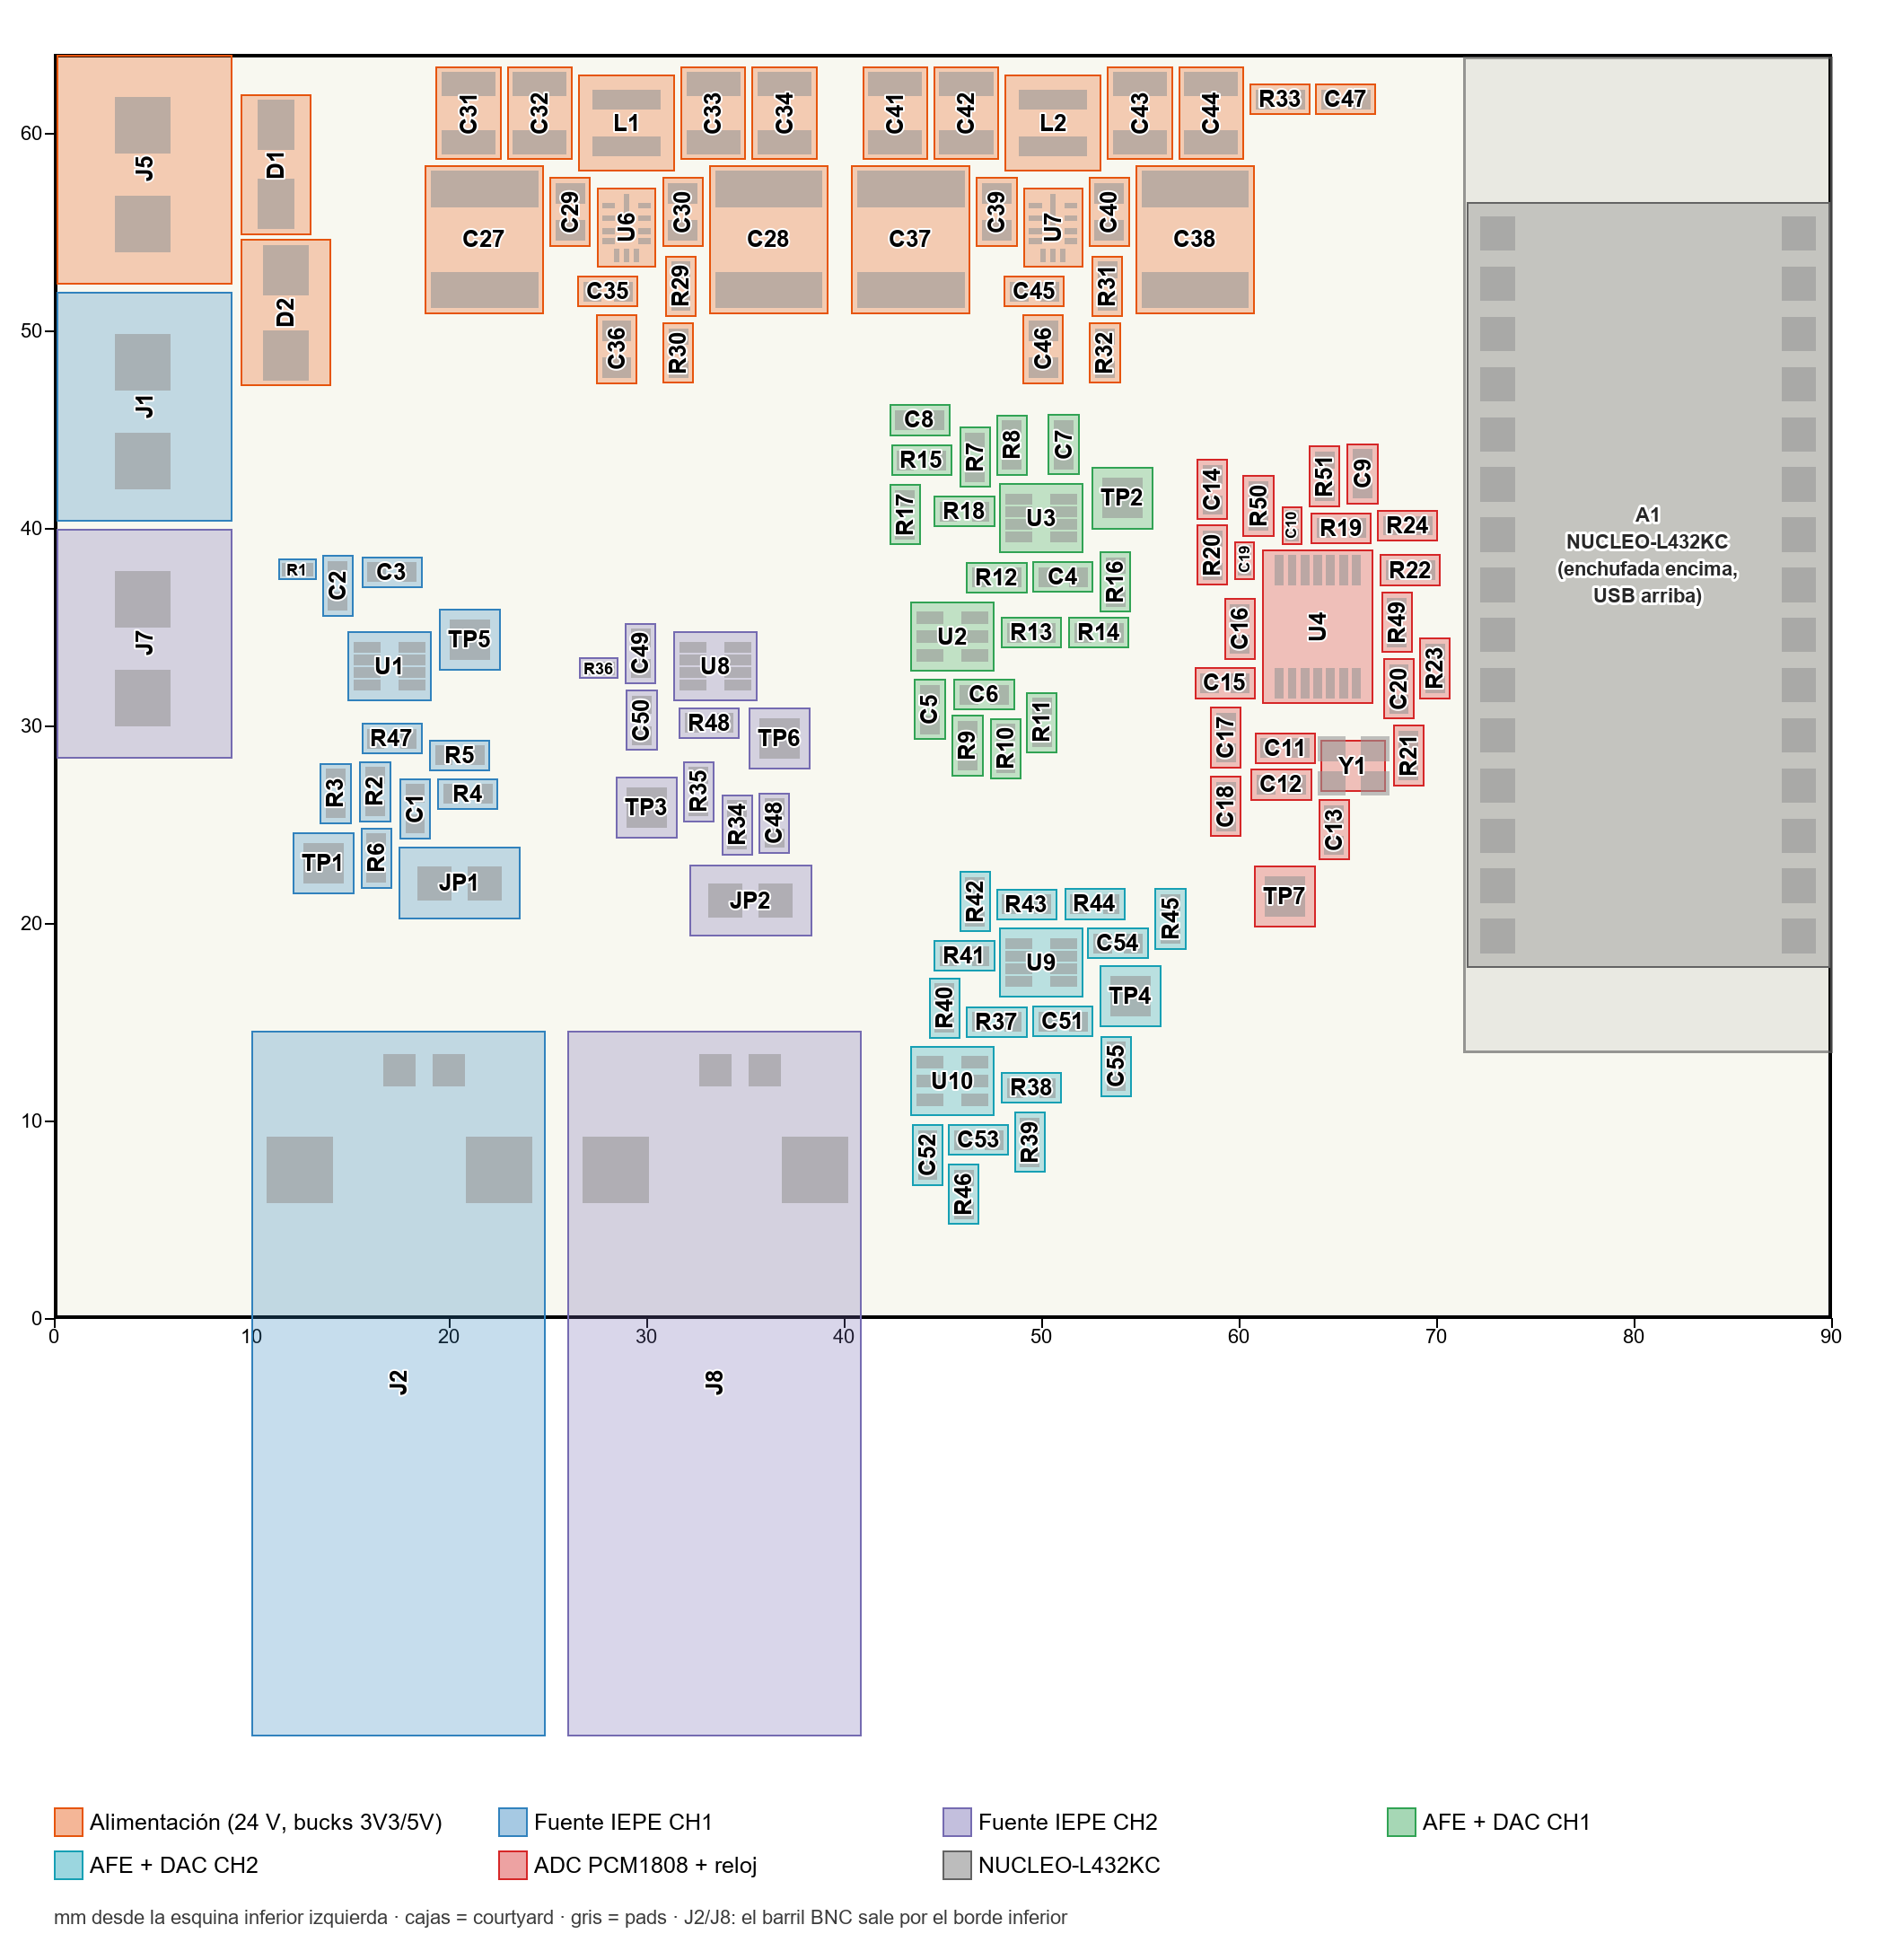
\includegraphics[width=\linewidth]{placement_map.png}\end{center}
\par\textbf{Al rutear}: U3 (AFE CH1, nodo SUM de 1 M$\Omega$ con R7/R18) queda unos 15 mm debajo del buck
U7/L2: no pasar SW\_5, SW\_3 ni los lazos de entrada de los bucks por encima de U3/U2/R13–R18, y dejar GND
entre ambos bloques. Plano de GND en la capa inferior (cosido con vías), lazos de entrada de los bucks
lo más cortos posible y lejos del AFE, y las señales analógicas (IEPE, REST, DC\_MON) lejos de los nodos SW.
Reglas de JLCPCB ya configuradas en el proyecto: 0.15 mm de separación, pistas de 0.2 mm (0.5 mm en la clase
\emph{Potencia}).
{\footnotesize\begin{longtable}{@{}llrrrl|llrrrl@{}}\toprule
\textbf{Ref} & \textbf{Valor} & \textbf{X} & \textbf{Y} & \textbf{Rot} & \textbf{Cara} & \textbf{Ref} & \textbf{Valor} & \textbf{X} & \textbf{Y} & \textbf{Rot} & \textbf{Cara}\\\midrule\endhead
A1 & NUCLEO-L432KC & 73.11 & 54.90 & 0 & sup & L1 & 6.8uH & 29.00 & 60.50 & 90 & sup\\
C1 & 100nF & 18.30 & 25.78 & 270 & sup & L2 & 10uH & 50.60 & 60.50 & 90 & sup\\
C2 & 1uF & 14.38 & 37.07 & 270 & sup & R1 & 10R & 12.34 & 37.90 & 0 & sup\\
C3 & 100nF & 17.13 & 37.76 & 0 & sup & R2 & 150R & 16.27 & 26.64 & 90 & sup\\
C4 & 100nF & 51.11 & 37.51 & 0 & sup & R3 & 150R & 14.27 & 26.56 & 90 & sup\\
C5 & 10uF & 44.36 & 30.80 & 270 & sup & R4 & 10k & 20.97 & 26.54 & 180 & sup\\
C6 & 100nF & 47.11 & 31.56 & 0 & sup & R5 & 10k & 20.56 & 28.50 & 0 & sup\\
C7 & 100nF & 51.14 & 44.22 & 270 & sup & R6 & 1k & 16.33 & 23.28 & 90 & sup\\
C8 & 100nF & 43.86 & 45.46 & 0 & sup & R7 & 49k9 & 46.65 & 43.58 & 90 & sup\\
C9 & 10uF & 66.27 & 42.75 & 270 & sup & R8 & 49k9 & 48.51 & 44.19 & 90 & sup\\
C10 & 10nF & 62.70 & 40.11 & 90 & sup & R9 & 100R & 46.27 & 28.98 & 270 & sup\\
C11 & 10uF & 62.35 & 28.85 & 180 & sup & R10 & 4k7 & 48.20 & 28.83 & 270 & sup\\
C12 & 100nF & 62.16 & 27.00 & 180 & sup & R11 & 4k7 & 50.04 & 30.15 & 270 & sup\\
C13 & 100nF & 64.83 & 24.71 & 270 & sup & R12 & 10k & 47.75 & 37.49 & 0 & sup\\
C14 & 10uF & 58.68 & 41.95 & 270 & sup & R13 & 390k & 49.50 & 34.70 & 0 & sup\\
C15 & 10uF & 59.30 & 32.14 & 180 & sup & R14 & 365k & 52.93 & 34.70 & 180 & sup\\
C16 & 100nF & 60.06 & 34.89 & 90 & sup & R15 & 10k & 43.93 & 43.42 & 0 & sup\\
C17 & 100nF & 59.35 & 29.39 & 270 & sup & R16 & 191k & 53.77 & 37.26 & 270 & sup\\
C18 & 10uF & 59.35 & 25.90 & 270 & sup & R17 & 10k & 43.11 & 40.67 & 90 & sup\\
C19 & 10nF & 60.30 & 38.36 & 90 & sup & R18 & 54k9 & 46.11 & 40.83 & 180 & sup\\
C20 & 100nF & 68.11 & 31.86 & 270 & sup & R19 & 100R & 65.20 & 40.00 & 180 & sup\\
C27 & 4.7uF & 21.80 & 54.60 & 90 & sup & R20 & 100R & 58.68 & 38.62 & 270 & sup\\
C28 & 4.7uF & 36.20 & 54.60 & 90 & sup & R21 & 100R & 68.60 & 28.48 & 90 & sup\\
C29 & 220nF & 26.15 & 56.00 & 90 & sup & R22 & 100R & 68.70 & 37.86 & 180 & sup\\
C30 & 220nF & 31.85 & 56.00 & 90 & sup & R23 & 100R & 69.95 & 32.89 & 270 & sup\\
C31 & 15uF & 21.00 & 61.00 & 270 & sup & R24 & 100R & 68.55 & 40.11 & 180 & sup\\
C32 & 15uF & 24.60 & 61.00 & 270 & sup & R29 & 100k & 31.75 & 52.24 & 270 & sup\\
C33 & 15uF & 33.40 & 61.00 & 270 & sup & R30 & 43.2k & 31.62 & 48.86 & 270 & sup\\
C34 & 15uF & 37.00 & 61.00 & 270 & sup & R31 & 100k & 53.35 & 52.24 & 270 & sup\\
C35 & 100nF & 28.05 & 51.96 & 180 & sup & R32 & 24.9k & 53.22 & 48.86 & 270 & sup\\
C36 & 2.2uF & 28.50 & 49.05 & 270 & sup & R33 & 10R & 62.10 & 61.69 & 0 & sup\\
C37 & 4.7uF & 43.40 & 54.60 & 90 & sup & R34 & 15k & 34.59 & 24.96 & 270 & sup\\
C38 & 4.7uF & 57.80 & 54.60 & 90 & sup & R35 & 100R & 32.65 & 26.64 & 270 & sup\\
C39 & 220nF & 47.75 & 56.00 & 90 & sup & R36 & 10R & 27.59 & 32.90 & 0 & sup\\
C40 & 220nF & 53.45 & 56.00 & 90 & sup & R37 & 10k & 47.75 & 14.99 & 0 & sup\\
C41 & 15uF & 42.60 & 61.00 & 270 & sup & R38 & 390k & 49.50 & 11.65 & 0 & sup\\
C42 & 15uF & 46.20 & 61.00 & 270 & sup & R39 & 365k & 49.43 & 8.90 & 90 & sup\\
C43 & 15uF & 55.00 & 61.00 & 270 & sup & R40 & 191k & 45.11 & 15.70 & 270 & sup\\
C44 & 15uF & 58.60 & 61.00 & 270 & sup & R41 & 54k9 & 46.11 & 18.32 & 180 & sup\\
C45 & 100nF & 49.65 & 51.96 & 180 & sup & R42 & 49k9 & 46.65 & 21.07 & 90 & sup\\
C46 & 2.2uF & 50.10 & 49.05 & 270 & sup & R43 & 49k9 & 49.26 & 20.94 & 180 & sup\\
C47 & 10uF & 65.42 & 61.69 & 0 & sup & R44 & 10k & 52.72 & 20.96 & 180 & sup\\
C48 & 100nF & 36.49 & 25.06 & 270 & sup & R45 & 10k & 56.55 & 20.21 & 90 & sup\\
C49 & 1uF & 29.71 & 33.65 & 90 & sup & R46 & 100R & 46.08 & 6.26 & 270 & sup\\
C50 & 100nF & 29.77 & 30.27 & 270 & sup & R47 & 180R & 17.13 & 29.33 & 0 & sup\\
C51 & 100nF & 51.11 & 15.01 & 0 & sup & R48 & 150R & 33.18 & 30.12 & 0 & sup\\
C52 & 10uF & 44.25 & 8.25 & 270 & sup & R49 & 10k & 68.01 & 35.22 & 90 & sup\\
C53 & 100nF & 46.83 & 9.01 & 0 & sup & R50 & 10k & 61.00 & 41.11 & 90 & sup\\
C54 & 100nF & 53.89 & 18.97 & 180 & sup & R51 & 10k & 64.35 & 42.61 & 90 & sup\\
C55 & 100nF & 53.80 & 12.74 & 270 & sup & U1 & LT3092ETS8\#TRP & 17.00 & 33.00 & 0 & sup\\
D1 & SS34 & 11.25 & 58.40 & 90 & sup & U2 & MCP4725A0T-E/C & 45.50 & 34.50 & 0 & sup\\
D2 & SMBJ26A & 11.75 & 50.90 & 270 & sup & U3 & TLV9062IDDFR & 50.00 & 40.50 & 0 & sup\\
J1 & EN\_\allowbreak{}IEPE\_\allowbreak{}CH1 & 4.50 & 48.40 & 270 & sup & U4 & PCM1808PW & 64.00 & 35.00 & 90 & sup\\
J2 & BNC\_\allowbreak{}MIC\_\allowbreak{}CH1 & 17.50 & 10.02 & 0 & sup & U6 & LMR36015FBRNXR & 29.00 & 55.20 & 0 & sup\\
J5 & 24V\_\allowbreak{}IN & 4.50 & 60.40 & 270 & sup & U7 & LMR36015FBRNXR & 50.60 & 55.20 & 0 & sup\\
J7 & EN\_\allowbreak{}IEPE\_\allowbreak{}CH2 & 4.50 & 36.40 & 270 & sup & U8 & LT3092ETS8\#TRP & 33.50 & 33.00 & 0 & sup\\
J8 & BNC\_\allowbreak{}MIC\_\allowbreak{}CH2 & 33.50 & 10.02 & 0 & sup & U9 & TLV9062IDDFR & 50.00 & 18.00 & 0 & sup\\
JP1 & STEP\_\allowbreak{}CH1 & 19.27 & 22.01 & 90 & sup & U10 & MCP4725A0T-E/C & 45.50 & 12.00 & 0 & sup\\
JP2 & STEP\_\allowbreak{}CH2 & 34.00 & 21.13 & 90 & sup & Y1 & 24.576MHz & 65.80 & 27.94 & 0 & sup\\
\bottomrule\end{longtable}}
Coordenadas en mm desde la esquina inferior izquierda (Y hacia arriba); rotación en grados (antihorario).
X/Y es el \textbf{origen del footprint de KiCad} (centro en las piezas SMD, pin 1 en conectores THT) y la rotación
es respecto a la orientación de la librería de KiCad: los footprints de Altium pueden tener otro origen o girar
distinto. Por eso, para las piezas con orientación, usa la tabla siguiente: si el \textbf{pad 1} de cada pieza
cae en ese punto y la pieza se ve como en el mapa, está bien puesta.
{\scriptsize\begin{longtable}{@{}llrr|llrr|llrr@{}}\toprule
\textbf{Ref} & \textbf{Valor} & \textbf{X p1} & \textbf{Y p1} & \textbf{Ref} & \textbf{Valor} & \textbf{X p1} & \textbf{Y p1} & \textbf{Ref} & \textbf{Valor} & \textbf{X p1} & \textbf{Y p1}\\\midrule\endhead
J5 & 24V\_\allowbreak{}IN & 4.50 & 60.40 & JP1 & STEP\_\allowbreak{}CH1 & 19.27 & 22.01 & U3 & TLV9062IDDFR & 48.86 & 41.47\\
D1 & SS34 & 11.25 & 56.40 & J2 & BNC\_\allowbreak{}MIC\_\allowbreak{}CH1 & 17.50 & 12.55 & U9 & TLV9062IDDFR & 48.86 & 18.97\\
D2 & SMBJ26A & 11.75 & 53.05 & J7 & EN\_\allowbreak{}IEPE\_\allowbreak{}CH2 & 4.50 & 36.40 & U10 & MCP4725A0T-E/ & 44.36 & 12.95\\
U6 & LMR36015FBRNX & 28.10 & 56.33 & U8 & LT3092ETS8\#TR & 32.36 & 33.97 & U4 & PCM1808PW & 62.05 & 32.14\\
U7 & LMR36015FBRNX & 49.70 & 56.33 & JP2 & STEP\_\allowbreak{}CH2 & 34.00 & 21.13 & Y1 & 24.576MHz & 64.70 & 27.06\\
J1 & EN\_\allowbreak{}IEPE\_\allowbreak{}CH1 & 4.50 & 48.40 & J8 & BNC\_\allowbreak{}MIC\_\allowbreak{}CH2 & 33.50 & 12.55 & A1 & NUCLEO-L432KC & 73.11 & 54.90\\
U1 & LT3092ETS8\#TR & 15.86 & 33.97 & U2 & MCP4725A0T-E/ & 44.36 & 35.45 & & & &\\
\bottomrule\end{longtable}}
\section{Cálculos de diseño}
\begin{longtable}{@{}L{0.27\linewidth}L{0.69\linewidth}@{}}\toprule
\textbf{Qué} & \textbf{Cálculo y resultado}\\\midrule\endhead
Corriente CH1 (RG-50) & I = 10 µA·(1 + R\_\allowbreak{}SET/R\_\allowbreak{}OUT) = 10 µA·(1 + 21 kΩ/75 Ω) = 2.81 mA. Con JP1: R\_\allowbreak{}OUT = 75 \ensuremath{\parallel} 180 = 52.9 Ω → 3.98 mA. RG-50 admite 2–20 mA.\\[2pt]
Corriente CH2 (SV 12L) & I = 10 µA·(1 + 15 kΩ/100 Ω) = 1.51 mA. Con JP2: 100 \ensuremath{\parallel} 150 = 60 Ω → 2.51 mA (2.5 mA es lo que le dan los equipos Svantek).\\[2pt]
Carga del AFE sobre el sensor & La cadena de 1 MΩ toma (V\_\allowbreak{}IEPE − VSHIFT)/1 MΩ \ensuremath{\approx} 9–10 µA: despreciable frente a mA.\\[2pt]
Margen de voltaje (compliance) & 24 V − 0.5 V (D1) − 0.03 V (R1) − 1.2 V (mínimo del LT3092) − 0.21 V (R\_\allowbreak{}OUT) \ensuremath{\approx} 22 V disponibles para el sensor. El RG-50 necesita 12.5 V de bias + 3.2 V pico \ensuremath{\approx} 16 V: sobran \ensuremath{\approx} 6 V.\\[2pt]
Protección de entrada & D1 SS34 (40 V, 3 A) bloquea la polaridad invertida. D2 SMBJ26A: no conduce a 24 V (V\_\allowbreak{}RWM = 26 V), ruptura \ensuremath{\geq} 28.9 V, recorte 42.1 V a 14.3 A (pulso 10/1000 µs).\\[2pt]
Punto de trabajo del restador & REST = 1.1·VSHIFT − 0.1·V\_\allowbreak{}IEPE. VSHIFT máx \ensuremath{\approx} 3.26 V (DAC a 3V3 menos la caída en R9). Con REST objetivo = 1.5 V se cubre cualquier bias de 0 a 20.9 V. Para el RG-50 (12.5 V): VSHIFT = 2.50 V. La señal (±0.32 V máx.) queda entre 1.18 y 1.82 V.\\[2pt]
Corrección del DC (firmware) & DC\_\allowbreak{}MON = REST/2 \ensuremath{\approx} 0.75 V. Si DC\_\allowbreak{}MON cambia más de un umbral: VSHIFT ← VSHIFT − 2·(DC\_\allowbreak{}MON − 0.75 V)/1.1, se escribe al DAC y se deja quieto mientras se mide (así no actúa como filtro pasa-altos).\\[2pt]
Resolución del DAC & 1 LSB = 0.80 mV en VSHIFT → 0.88 mV en REST.\\[2pt]
Rapidez del lazo & Filtro del DAC: 10 kΩ·100 nF = 1 ms (antes 100 ms). Filtro de DC\_\allowbreak{}MON: 5 kΩ·100 nF = 0.5 ms (antes 50 ms). La corrección completa tarda unos milisegundos.\\[2pt]
Acople al ADC & C9/C14 = 10 µF con 60 kΩ de entrada del PCM1808 → f\_\allowbreak{}c = 0.26 Hz. El PCM1808 tiene además un pasa-altos interno de 0.019·fs/1000 = 0.91 Hz a 48 kHz (no se puede desactivar). Desfase total a 20 Hz \ensuremath{\approx} 3.4°.\\[2pt]
Reloj & 24.576 MHz = 512 × 48 kHz: PCM1808 maestro 512 fs → fs = 48 kHz, BCK = 64 fs = 3.072 MHz.\\[2pt]
Niveles en el ADC & Fondo de escala 3 Vpp = 1.06 Vrms. RG-50 (50 mV/Pa nominal): 94 dB SPL → 5 mVrms en el ADC (−46.5 dBFS); 130 dB pico → 0.32 V pico: nunca satura.\\[2pt]
Ruido / límite & SNR del PCM1808 = 99 dB → 12 µVrms en el ADC \ensuremath{\approx} 41.5 dB SPL referido al micrófono. Limitación honesta: la ganancia 0.1 desaprovecha \ensuremath{\approx} 13 dB del ADC.\\[2pt]
Consumo (estimado) & 3V3: PCM1808 5.9 mA + oscilador + 2 DAC + pull-ups \ensuremath{\approx} 15–20 mA. 5V\_\allowbreak{}A: PCM1808 8.6 mA + 2 TLV9062 \ensuremath{\approx} 11 mA (caída en R33 \ensuremath{\approx} 0.1 V). Entrada 24 V: \ensuremath{\approx} 10–15 mA en total. Fuente de laboratorio con límite de 50 mA.\\[2pt]
\bottomrule\end{longtable}
\section{Pruebas y demostración}
\begin{longtable}{@{}L{0.2\linewidth}L{0.76\linewidth}@{}}\toprule
0. Antes de pedir & Alimentar la placa del gateway y medir con osciloscopio 3V3 y 5V y su rizado: valida el bloque de bucks que se copia.\\[2pt]
1. Llega la placa & Fuente a 24 V con límite de 50 mA, sin NUCLEO ni micrófonos: medir 3V3, 5V y 5V\_A.\\[2pt]
2. Fuentes IEPE & Amperímetro en lugar del puente J1/J7 y ~4.7 kΩ en el BNC: 2.81 mA y 1.51 mA; con JP1/JP2 \ensuremath{\approx} 3.98 y 2.51 mA.\\[2pt]
3. Micrófono falso & Zener de 12 V en el BNC + generador (1 kHz) por un condensador: en TP1 \ensuremath{\approx} 12 V DC + la onda; en TP2 la onda × 0.1 sobre un DC fijo.\\[2pt]
4. NUCLEO y lazo & Enchufar la NUCLEO (USB primero, luego 24 V), cargar firmware, poner/quitar JP1: REST salta y vuelve a 1.5 V en milisegundos.\\[2pt]
5. ADC al PC & Capturar I$^2$S y graficar en Python: onda de 1 kHz sin DC y su FFT.\\[2pt]
6. Micrófonos & RG-50 en J2; SV 12L en J8 con adaptador BNC–TNC. Medir el bias real en TP1/TP3.\\[2pt]
\bottomrule\end{longtable}
\textbf{Demo para el profesor:} (1) osciloscopio en TP1: DC del sensor con la señal encima; (2) en TP2: la
misma señal sin el DC del sensor (sobre el punto de trabajo fijo de 1.5 V), sin condensador en el camino;
(3) poner JP1: la corriente sube de 2.81 a 3.98 mA, se ve el salto y el DAC lo corrige en milisegundos;
(4) la señal digitalizada en el PC.
\textbf{Ojo con el paso (3):} un sensor IEPE fija su propio voltaje de bias, así que con el micrófono real
el salto de corriente casi no mueve el DC (se ve poco). Para que el salto sea grande y claro, hacer esa parte
con la \textbf{resistencia de 4.7 k$\Omega$} en el BNC (V = I·R): 2.81 mA → 13.2 V y 3.98 mA → 18.7 V, un
escalón de 5.5 V en TP1 y de −0.55 V en TP2 antes de que el DAC lo corrija (VSHIFT pasa de 2.56 a 3.06 V,
dentro de su rango). Luego se repite con el micrófono y se mide cuánto cambia su bias en realidad.
\section{Pendientes y riesgos (honesto)}
\begin{itemize}
\item Ruteo: no está hecho. La prueba con autorruteador (Freerouting) no se pudo correr en esta sesión; el script \texttt{tools/probar\_ruteo.sh} la hace. Estimado: 246 conexiones, \ensuremath{\approx} 1.26 m de ratsnest, 76 cruces fuera de GND.
\item LT3092: los valores de 1.2–40 V, 10 µA ±1 \% y 0.5–200 mA salen de las características del datasheet (copia de terceros); analog.com no fue accesible. Confirmar con el PDF oficial.
\item Footprint RNX0012A (U6/U7): coincide con el de JLC (C1850339) salvo rotación de 90° y 0.14 mm de origen: revisar la vista previa del CPL de JLC.
\item Stock en LCSC: LMR36015FBRNXR tenía poco stock (12–21 unidades cuando se consultó); revisar el día del pedido.
\item Piezas JLC sin código LCSC en el diseño (heredadas del Altium y del gateway): L1, C27, C28, C29, C30, C31, C32, C33, C34, C36, R29, R30, L2, C37, C38, C39, C40, C41, C42, C43, C44, C46, R31, R32, R33, R1, R36, R34, R35, C10, C19. JLC las busca por MPN al subir el BOM; si no las tiene, elegir un equivalente (mismo valor, tamaño y tensión). Los códigos con * de la tabla de componentes se hallaron por búsqueda web.
\item BNC Kinghelm de 75 Ω: para audio la impedancia no importa y acopla con BNC de 50 Ω.
\item Ganancia 0.1 del restador: limita el ruido equivalente a \ensuremath{\approx} 41.5 dB SPL (aceptable para el laboratorio).
\item Firmware pendiente: SAI (I$^2$S esclavo), ADC (DC\_MON), I$^2$C a los DAC, lazo de corrección y envío al PC.
\end{itemize}
\end{document}